\documentclass[twoside]{book}

% Packages required by doxygen
\usepackage{fixltx2e}
\usepackage{calc}
\usepackage{doxygen}
\usepackage[export]{adjustbox} % also loads graphicx
\usepackage{graphicx}
\usepackage[utf8]{inputenc}
\usepackage{makeidx}
\usepackage{multicol}
\usepackage{multirow}
\PassOptionsToPackage{warn}{textcomp}
\usepackage{textcomp}
\usepackage[nointegrals]{wasysym}
\usepackage[table]{xcolor}

% NLS support packages
\usepackage[T2A]{fontenc}
\usepackage[russian]{babel}

% Font selection
\usepackage[T1]{fontenc}
\usepackage[scaled=.90]{helvet}
\usepackage{courier}
\usepackage{amssymb}
\usepackage{sectsty}
\renewcommand{\familydefault}{\sfdefault}
\allsectionsfont{%
  \fontseries{bc}\selectfont%
  \color{darkgray}%
}
\renewcommand{\DoxyLabelFont}{%
  \fontseries{bc}\selectfont%
  \color{darkgray}%
}
\newcommand{\+}{\discretionary{\mbox{\scriptsize$\hookleftarrow$}}{}{}}

% Page & text layout
\usepackage{geometry}
\geometry{%
  a4paper,%
  top=2.5cm,%
  bottom=2.5cm,%
  left=2.5cm,%
  right=2.5cm%
}
\tolerance=750
\hfuzz=15pt
\hbadness=750
\setlength{\emergencystretch}{15pt}
\setlength{\parindent}{0cm}
\setlength{\parskip}{0.2cm}
\makeatletter
\renewcommand{\paragraph}{%
  \@startsection{paragraph}{4}{0ex}{-1.0ex}{1.0ex}{%
    \normalfont\normalsize\bfseries\SS@parafont%
  }%
}
\renewcommand{\subparagraph}{%
  \@startsection{subparagraph}{5}{0ex}{-1.0ex}{1.0ex}{%
    \normalfont\normalsize\bfseries\SS@subparafont%
  }%
}
\makeatother

% Headers & footers
\usepackage{fancyhdr}
\pagestyle{fancyplain}
\fancyhead[LE]{\fancyplain{}{\bfseries\thepage}}
\fancyhead[CE]{\fancyplain{}{}}
\fancyhead[RE]{\fancyplain{}{\bfseries\leftmark}}
\fancyhead[LO]{\fancyplain{}{\bfseries\rightmark}}
\fancyhead[CO]{\fancyplain{}{}}
\fancyhead[RO]{\fancyplain{}{\bfseries\thepage}}
\fancyfoot[LE]{\fancyplain{}{}}
\fancyfoot[CE]{\fancyplain{}{}}
\fancyfoot[RE]{\fancyplain{}{\bfseries\scriptsize Документация по Q\+Tester\+\_\+client. Последние изменения\+: Пт 17 Апр 2015 03\+:09\+:57. Создано системой Doxygen }}
\fancyfoot[LO]{\fancyplain{}{\bfseries\scriptsize Документация по Q\+Tester\+\_\+client. Последние изменения\+: Пт 17 Апр 2015 03\+:09\+:57. Создано системой Doxygen }}
\fancyfoot[CO]{\fancyplain{}{}}
\fancyfoot[RO]{\fancyplain{}{}}
\renewcommand{\footrulewidth}{0.4pt}
\renewcommand{\chaptermark}[1]{%
  \markboth{#1}{}%
}
\renewcommand{\sectionmark}[1]{%
  \markright{\thesection\ #1}%
}

% Indices & bibliography
\usepackage{natbib}
\usepackage[titles]{tocloft}
\setcounter{tocdepth}{3}
\setcounter{secnumdepth}{5}
\makeindex

% Hyperlinks (required, but should be loaded last)
\usepackage{ifpdf}
\ifpdf
  \usepackage[pdftex,pagebackref=true]{hyperref}
\else
  \usepackage[ps2pdf,pagebackref=true]{hyperref}
\fi
\hypersetup{%
  colorlinks=true,%
  linkcolor=blue,%
  citecolor=blue,%
  unicode%
}

% Custom commands
\newcommand{\clearemptydoublepage}{%
  \newpage{\pagestyle{empty}\cleardoublepage}%
}


%===== C O N T E N T S =====

\begin{document}

% Titlepage & ToC
\hypersetup{pageanchor=false,
             bookmarks=true,
             bookmarksnumbered=true,
             pdfencoding=unicode
            }
\pagenumbering{roman}
\begin{titlepage}
\vspace*{7cm}
\begin{center}%
{\Large Q\+Tester\+\_\+client \\[1ex]\large 0.\+2 }\\
\vspace*{1cm}
{\large Создано системой Doxygen 1.8.9.1}\\
\vspace*{0.5cm}
{\small Пт 17 Апр 2015 03:09:57}\\
\end{center}
\end{titlepage}
\clearemptydoublepage
\tableofcontents
\clearemptydoublepage
\pagenumbering{arabic}
\hypersetup{pageanchor=true}

%--- Begin generated contents ---
\chapter{Иерархический список классов}
\section{Иерархия классов}
Иерархия классов.\begin{DoxyCompactList}
\item \contentsline{section}{Account}{\pageref{class_account}}{}
\begin{DoxyCompactList}
\item \contentsline{section}{User}{\pageref{class_user}}{}
\begin{DoxyCompactList}
\item \contentsline{section}{Student}{\pageref{class_student}}{}
\item \contentsline{section}{Teacher}{\pageref{class_teacher}}{}
\end{DoxyCompactList}
\end{DoxyCompactList}
\item \contentsline{section}{S\+Q\+L\+Mgr}{\pageref{class_s_q_l_mgr}}{}
\begin{DoxyCompactList}
\item \contentsline{section}{S\+Q\+Lite\+Mgr}{\pageref{class_s_q_lite_mgr}}{}
\end{DoxyCompactList}
\item \contentsline{section}{Tester}{\pageref{class_tester}}{}
\item \contentsline{section}{Test\+Generator}{\pageref{class_test_generator}}{}
\item \contentsline{section}{U\+A\+C}{\pageref{class_u_a_c}}{}
\item \contentsline{section}{User\+Group}{\pageref{class_user_group}}{}
\begin{DoxyCompactList}
\item \contentsline{section}{Administrator}{\pageref{class_administrator}}{}
\begin{DoxyCompactList}
\item \contentsline{section}{Base\+Manager}{\pageref{class_base_manager}}{}
\item \contentsline{section}{Examenator}{\pageref{class_examenator}}{}
\end{DoxyCompactList}
\item \contentsline{section}{Examiner}{\pageref{class_examiner}}{}
\end{DoxyCompactList}
\end{DoxyCompactList}

\chapter{Алфавитный указатель классов}
\section{Классы}
Классы с их кратким описанием.\begin{DoxyCompactList}
\item\contentsline{section}{\hyperlink{class_account}{Account} }{\pageref{db/d22/class_account}}{}
\item\contentsline{section}{\hyperlink{class_administrator}{Administrator} }{\pageref{dd/d29/class_administrator}}{}
\item\contentsline{section}{\hyperlink{class_base_manager}{Base\+Manager} }{\pageref{d8/dc6/class_base_manager}}{}
\item\contentsline{section}{\hyperlink{class_examenator}{Examenator} }{\pageref{d9/d7c/class_examenator}}{}
\item\contentsline{section}{\hyperlink{class_examiner}{Examiner} }{\pageref{d6/d26/class_examiner}}{}
\item\contentsline{section}{\hyperlink{class_s_q_lite_mgr}{S\+Q\+Lite\+Mgr} }{\pageref{dc/da5/class_s_q_lite_mgr}}{}
\item\contentsline{section}{\hyperlink{class_s_q_l_mgr}{S\+Q\+L\+Mgr} }{\pageref{df/dd0/class_s_q_l_mgr}}{}
\item\contentsline{section}{\hyperlink{class_student}{Student} }{\pageref{db/d66/class_student}}{}
\item\contentsline{section}{\hyperlink{class_teacher}{Teacher} }{\pageref{dc/d2d/class_teacher}}{}
\item\contentsline{section}{\hyperlink{class_tester}{Tester} }{\pageref{d9/d27/class_tester}}{}
\item\contentsline{section}{\hyperlink{class_test_generator}{Test\+Generator} }{\pageref{db/d4d/class_test_generator}}{}
\item\contentsline{section}{\hyperlink{class_u_a_c}{U\+A\+C} }{\pageref{d3/d61/class_u_a_c}}{}
\item\contentsline{section}{\hyperlink{class_user}{User} }{\pageref{d7/d23/class_user}}{}
\item\contentsline{section}{\hyperlink{class_user_group}{User\+Group} }{\pageref{d8/d7e/class_user_group}}{}
\end{DoxyCompactList}

\chapter{Список файлов}
\section{Файлы}
Полный список файлов.\begin{DoxyCompactList}
\item\contentsline{section}{Q\+Tester\+\_\+client/\+Q\+Tester\+\_\+client/\hyperlink{_account_8cpp}{Account.\+cpp} }{\pageref{de/d9a/_account_8cpp}}{}
\item\contentsline{section}{Q\+Tester\+\_\+client/\+Q\+Tester\+\_\+client/\hyperlink{_account_8h}{Account.\+h} }{\pageref{d6/d5f/_account_8h}}{}
\item\contentsline{section}{Q\+Tester\+\_\+client/\+Q\+Tester\+\_\+client/\hyperlink{_administrator_8cpp}{Administrator.\+cpp} }{\pageref{d7/db7/_administrator_8cpp}}{}
\item\contentsline{section}{Q\+Tester\+\_\+client/\+Q\+Tester\+\_\+client/\hyperlink{_administrator_8h}{Administrator.\+h} }{\pageref{de/dcc/_administrator_8h}}{}
\item\contentsline{section}{Q\+Tester\+\_\+client/\+Q\+Tester\+\_\+client/\hyperlink{_base_manager_8cpp}{Base\+Manager.\+cpp} }{\pageref{d9/d4e/_base_manager_8cpp}}{}
\item\contentsline{section}{Q\+Tester\+\_\+client/\+Q\+Tester\+\_\+client/\hyperlink{_base_manager_8h}{Base\+Manager.\+h} }{\pageref{df/d6a/_base_manager_8h}}{}
\item\contentsline{section}{Q\+Tester\+\_\+client/\+Q\+Tester\+\_\+client/\hyperlink{_examenator_8cpp}{Examenator.\+cpp} }{\pageref{db/d7a/_examenator_8cpp}}{}
\item\contentsline{section}{Q\+Tester\+\_\+client/\+Q\+Tester\+\_\+client/\hyperlink{_examenator_8h}{Examenator.\+h} }{\pageref{da/da2/_examenator_8h}}{}
\item\contentsline{section}{Q\+Tester\+\_\+client/\+Q\+Tester\+\_\+client/\hyperlink{_examiner_8cpp}{Examiner.\+cpp} }{\pageref{de/d6b/_examiner_8cpp}}{}
\item\contentsline{section}{Q\+Tester\+\_\+client/\+Q\+Tester\+\_\+client/\hyperlink{_examiner_8h}{Examiner.\+h} }{\pageref{dd/d77/_examiner_8h}}{}
\item\contentsline{section}{Q\+Tester\+\_\+client/\+Q\+Tester\+\_\+client/\hyperlink{main_8cpp}{main.\+cpp} }{\pageref{df/d0a/main_8cpp}}{}
\item\contentsline{section}{Q\+Tester\+\_\+client/\+Q\+Tester\+\_\+client/\hyperlink{_s_q_lite_mgr_8cpp}{S\+Q\+Lite\+Mgr.\+cpp} }{\pageref{df/d58/_s_q_lite_mgr_8cpp}}{}
\item\contentsline{section}{Q\+Tester\+\_\+client/\+Q\+Tester\+\_\+client/\hyperlink{_s_q_lite_mgr_8h}{S\+Q\+Lite\+Mgr.\+h} }{\pageref{dd/dff/_s_q_lite_mgr_8h}}{}
\item\contentsline{section}{Q\+Tester\+\_\+client/\+Q\+Tester\+\_\+client/\hyperlink{_s_q_l_mgr_8cpp}{S\+Q\+L\+Mgr.\+cpp} }{\pageref{d5/d93/_s_q_l_mgr_8cpp}}{}
\item\contentsline{section}{Q\+Tester\+\_\+client/\+Q\+Tester\+\_\+client/\hyperlink{_s_q_l_mgr_8h}{S\+Q\+L\+Mgr.\+h} }{\pageref{dc/d5e/_s_q_l_mgr_8h}}{}
\item\contentsline{section}{Q\+Tester\+\_\+client/\+Q\+Tester\+\_\+client/\hyperlink{std_headers_8cpp}{std\+Headers.\+cpp} }{\pageref{d4/d3a/std_headers_8cpp}}{}
\item\contentsline{section}{Q\+Tester\+\_\+client/\+Q\+Tester\+\_\+client/\hyperlink{std_headers_8h}{std\+Headers.\+h} }{\pageref{df/d29/std_headers_8h}}{}
\item\contentsline{section}{Q\+Tester\+\_\+client/\+Q\+Tester\+\_\+client/\hyperlink{_student_8cpp}{Student.\+cpp} }{\pageref{db/d78/_student_8cpp}}{}
\item\contentsline{section}{Q\+Tester\+\_\+client/\+Q\+Tester\+\_\+client/\hyperlink{_student_8h}{Student.\+h} }{\pageref{d1/dbc/_student_8h}}{}
\item\contentsline{section}{Q\+Tester\+\_\+client/\+Q\+Tester\+\_\+client/\hyperlink{_teacher_8cpp}{Teacher.\+cpp} }{\pageref{d9/d15/_teacher_8cpp}}{}
\item\contentsline{section}{Q\+Tester\+\_\+client/\+Q\+Tester\+\_\+client/\hyperlink{_teacher_8h}{Teacher.\+h} }{\pageref{d2/d3f/_teacher_8h}}{}
\item\contentsline{section}{Q\+Tester\+\_\+client/\+Q\+Tester\+\_\+client/\hyperlink{_tester_8cpp}{Tester.\+cpp} }{\pageref{dd/d75/_tester_8cpp}}{}
\item\contentsline{section}{Q\+Tester\+\_\+client/\+Q\+Tester\+\_\+client/\hyperlink{_tester_8h}{Tester.\+h} }{\pageref{d1/d75/_tester_8h}}{}
\item\contentsline{section}{Q\+Tester\+\_\+client/\+Q\+Tester\+\_\+client/\hyperlink{_test_generator_8cpp}{Test\+Generator.\+cpp} }{\pageref{d5/dec/_test_generator_8cpp}}{}
\item\contentsline{section}{Q\+Tester\+\_\+client/\+Q\+Tester\+\_\+client/\hyperlink{_test_generator_8h}{Test\+Generator.\+h} }{\pageref{d1/d85/_test_generator_8h}}{}
\item\contentsline{section}{Q\+Tester\+\_\+client/\+Q\+Tester\+\_\+client/\hyperlink{_u_a_c_8cpp}{U\+A\+C.\+cpp} }{\pageref{de/d75/_u_a_c_8cpp}}{}
\item\contentsline{section}{Q\+Tester\+\_\+client/\+Q\+Tester\+\_\+client/\hyperlink{_u_a_c_8h}{U\+A\+C.\+h} }{\pageref{d0/d00/_u_a_c_8h}}{}
\item\contentsline{section}{Q\+Tester\+\_\+client/\+Q\+Tester\+\_\+client/\hyperlink{_user_8cpp}{User.\+cpp} }{\pageref{dc/d89/_user_8cpp}}{}
\item\contentsline{section}{Q\+Tester\+\_\+client/\+Q\+Tester\+\_\+client/\hyperlink{_user_8h}{User.\+h} }{\pageref{d3/d75/_user_8h}}{}
\item\contentsline{section}{Q\+Tester\+\_\+client/\+Q\+Tester\+\_\+client/\hyperlink{_user_group_8cpp}{User\+Group.\+cpp} }{\pageref{d8/df6/_user_group_8cpp}}{}
\item\contentsline{section}{Q\+Tester\+\_\+client/\+Q\+Tester\+\_\+client/\hyperlink{_user_group_8h}{User\+Group.\+h} }{\pageref{d6/d00/_user_group_8h}}{}
\end{DoxyCompactList}

\chapter{Классы}
\hypertarget{class_account}{}\section{Класс Account}
\label{class_account}\index{Account@{Account}}


{\ttfamily \#include $<$Account.\+h$>$}



Граф наследования\+:Account\+:\nopagebreak
\begin{figure}[H]
\begin{center}
\leavevmode
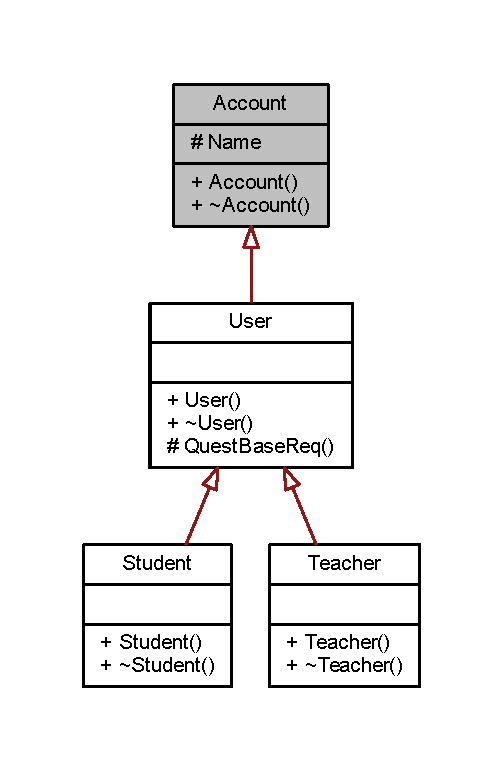
\includegraphics[width=242pt]{d6/d83/class_account__inherit__graph}
\end{center}
\end{figure}


Граф связей класса Account\+:\nopagebreak
\begin{figure}[H]
\begin{center}
\leavevmode
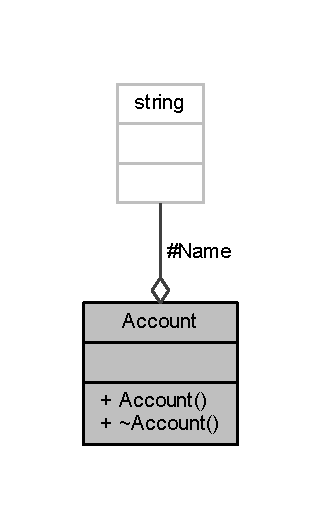
\includegraphics[width=154pt]{d5/d1b/class_account__coll__graph}
\end{center}
\end{figure}
\subsection*{Открытые члены}
\begin{DoxyCompactItemize}
\item 
\hyperlink{class_account_a366660970b5eeb5c17436062327f1b14}{Account} ()
\item 
\hyperlink{class_account_a569c9ef0e42b9157690b4ceb646daba8}{$\sim$\+Account} ()
\end{DoxyCompactItemize}
\subsection*{Защищенные данные}
\begin{DoxyCompactItemize}
\item 
string \hyperlink{class_account_af13e63ff7407ac19e41e91afc40185b7}{Name}
\end{DoxyCompactItemize}


\subsection{Подробное описание}


См. определение в файле Account.\+h строка 4



\subsection{Конструктор(ы)}
\hypertarget{class_account_a366660970b5eeb5c17436062327f1b14}{}\index{Account@{Account}!Account@{Account}}
\index{Account@{Account}!Account@{Account}}
\subsubsection[{Account}]{\setlength{\rightskip}{0pt plus 5cm}Account\+::\+Account (
\begin{DoxyParamCaption}
{}
\end{DoxyParamCaption}
)}\label{class_account_a366660970b5eeb5c17436062327f1b14}


См. определение в файле Account.\+cpp строка 4

\hypertarget{class_account_a569c9ef0e42b9157690b4ceb646daba8}{}\index{Account@{Account}!````~Account@{$\sim$\+Account}}
\index{````~Account@{$\sim$\+Account}!Account@{Account}}
\subsubsection[{$\sim$\+Account}]{\setlength{\rightskip}{0pt plus 5cm}Account\+::$\sim$\+Account (
\begin{DoxyParamCaption}
{}
\end{DoxyParamCaption}
)}\label{class_account_a569c9ef0e42b9157690b4ceb646daba8}


См. определение в файле Account.\+cpp строка 9



\subsection{Данные класса}
\hypertarget{class_account_af13e63ff7407ac19e41e91afc40185b7}{}\index{Account@{Account}!Name@{Name}}
\index{Name@{Name}!Account@{Account}}
\subsubsection[{Name}]{\setlength{\rightskip}{0pt plus 5cm}string Account\+::\+Name\hspace{0.3cm}{\ttfamily [protected]}}\label{class_account_af13e63ff7407ac19e41e91afc40185b7}


См. определение в файле Account.\+h строка 7



Объявления и описания членов классов находятся в файлах\+:\begin{DoxyCompactItemize}
\item 
Q\+Tester\+\_\+client/\+Q\+Tester\+\_\+client/\hyperlink{_account_8h}{Account.\+h}\item 
Q\+Tester\+\_\+client/\+Q\+Tester\+\_\+client/\hyperlink{_account_8cpp}{Account.\+cpp}\end{DoxyCompactItemize}

\hypertarget{class_administrator}{}\section{Класс Administrator}
\label{class_administrator}\index{Administrator@{Administrator}}


{\ttfamily \#include $<$Administrator.\+h$>$}



Граф наследования\+:Administrator\+:\nopagebreak
\begin{figure}[H]
\begin{center}
\leavevmode
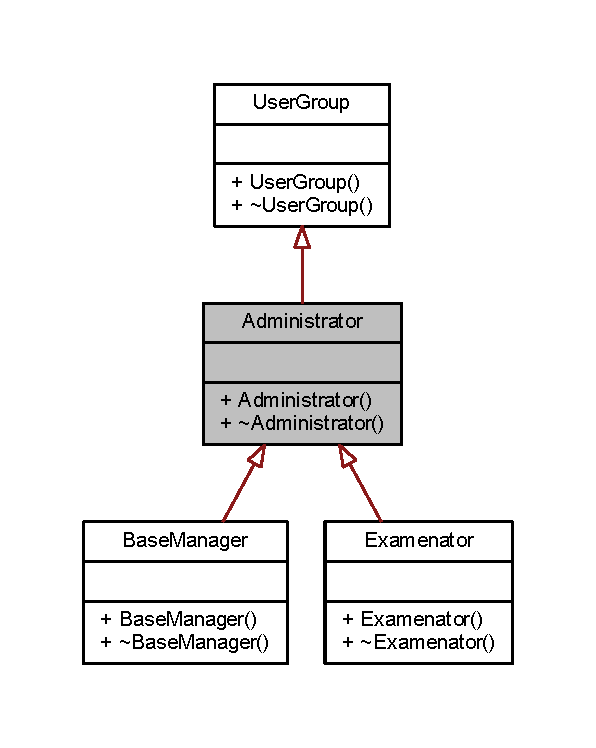
\includegraphics[width=286pt]{df/dc2/class_administrator__inherit__graph}
\end{center}
\end{figure}


Граф связей класса Administrator\+:\nopagebreak
\begin{figure}[H]
\begin{center}
\leavevmode
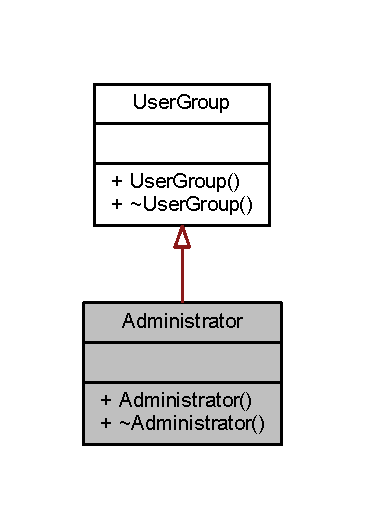
\includegraphics[width=175pt]{de/db4/class_administrator__coll__graph}
\end{center}
\end{figure}
\subsection*{Открытые члены}
\begin{DoxyCompactItemize}
\item 
\hyperlink{class_administrator_a2fe0bc295b84c5c49f5ff91c90d40e59}{Administrator} ()
\item 
\hyperlink{class_administrator_af5ce6d3689295045ed589a912853cacc}{$\sim$\+Administrator} ()
\end{DoxyCompactItemize}
\subsection*{Дополнительные унаследованные члены}


\subsection{Подробное описание}


См. определение в файле Administrator.\+h строка 3



\subsection{Конструктор(ы)}
\hypertarget{class_administrator_a2fe0bc295b84c5c49f5ff91c90d40e59}{}\index{Administrator@{Administrator}!Administrator@{Administrator}}
\index{Administrator@{Administrator}!Administrator@{Administrator}}
\subsubsection[{Administrator}]{\setlength{\rightskip}{0pt plus 5cm}Administrator\+::\+Administrator (
\begin{DoxyParamCaption}
{}
\end{DoxyParamCaption}
)}\label{class_administrator_a2fe0bc295b84c5c49f5ff91c90d40e59}


См. определение в файле Administrator.\+cpp строка 4

\hypertarget{class_administrator_af5ce6d3689295045ed589a912853cacc}{}\index{Administrator@{Administrator}!````~Administrator@{$\sim$\+Administrator}}
\index{````~Administrator@{$\sim$\+Administrator}!Administrator@{Administrator}}
\subsubsection[{$\sim$\+Administrator}]{\setlength{\rightskip}{0pt plus 5cm}Administrator\+::$\sim$\+Administrator (
\begin{DoxyParamCaption}
{}
\end{DoxyParamCaption}
)}\label{class_administrator_af5ce6d3689295045ed589a912853cacc}


См. определение в файле Administrator.\+cpp строка 9



Объявления и описания членов классов находятся в файлах\+:\begin{DoxyCompactItemize}
\item 
Q\+Tester\+\_\+client/\+Q\+Tester\+\_\+client/\hyperlink{_administrator_8h}{Administrator.\+h}\item 
Q\+Tester\+\_\+client/\+Q\+Tester\+\_\+client/\hyperlink{_administrator_8cpp}{Administrator.\+cpp}\end{DoxyCompactItemize}

\hypertarget{class_base_manager}{}\section{Класс Base\+Manager}
\label{class_base_manager}\index{Base\+Manager@{Base\+Manager}}


{\ttfamily \#include $<$Base\+Manager.\+h$>$}



Граф наследования\+:Base\+Manager\+:\nopagebreak
\begin{figure}[H]
\begin{center}
\leavevmode
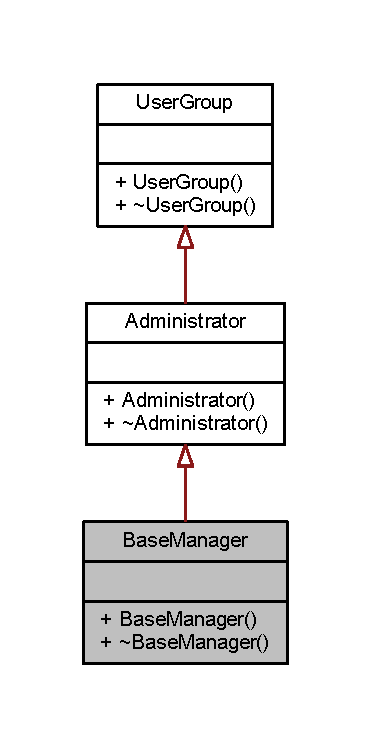
\includegraphics[width=178pt]{d9/db8/class_base_manager__inherit__graph}
\end{center}
\end{figure}


Граф связей класса Base\+Manager\+:\nopagebreak
\begin{figure}[H]
\begin{center}
\leavevmode
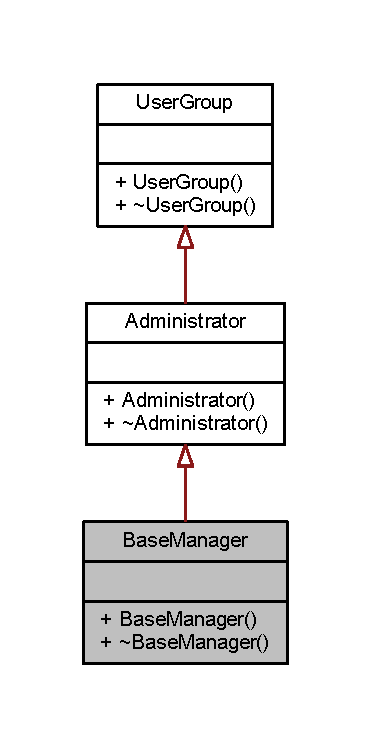
\includegraphics[width=178pt]{d8/d95/class_base_manager__coll__graph}
\end{center}
\end{figure}
\subsection*{Открытые члены}
\begin{DoxyCompactItemize}
\item 
\hyperlink{class_base_manager_a663ef30d41792bdecf2598a6285cfddd}{Base\+Manager} ()
\item 
\hyperlink{class_base_manager_af512e2d3b2a7727a2766a6c95a6b90a3}{$\sim$\+Base\+Manager} ()
\end{DoxyCompactItemize}
\subsection*{Дополнительные унаследованные члены}


\subsection{Подробное описание}


См. определение в файле Base\+Manager.\+h строка 3



\subsection{Конструктор(ы)}
\hypertarget{class_base_manager_a663ef30d41792bdecf2598a6285cfddd}{}\index{Base\+Manager@{Base\+Manager}!Base\+Manager@{Base\+Manager}}
\index{Base\+Manager@{Base\+Manager}!Base\+Manager@{Base\+Manager}}
\subsubsection[{Base\+Manager}]{\setlength{\rightskip}{0pt plus 5cm}Base\+Manager\+::\+Base\+Manager (
\begin{DoxyParamCaption}
{}
\end{DoxyParamCaption}
)}\label{class_base_manager_a663ef30d41792bdecf2598a6285cfddd}


См. определение в файле Base\+Manager.\+cpp строка 4

\hypertarget{class_base_manager_af512e2d3b2a7727a2766a6c95a6b90a3}{}\index{Base\+Manager@{Base\+Manager}!````~Base\+Manager@{$\sim$\+Base\+Manager}}
\index{````~Base\+Manager@{$\sim$\+Base\+Manager}!Base\+Manager@{Base\+Manager}}
\subsubsection[{$\sim$\+Base\+Manager}]{\setlength{\rightskip}{0pt plus 5cm}Base\+Manager\+::$\sim$\+Base\+Manager (
\begin{DoxyParamCaption}
{}
\end{DoxyParamCaption}
)}\label{class_base_manager_af512e2d3b2a7727a2766a6c95a6b90a3}


См. определение в файле Base\+Manager.\+cpp строка 9



Объявления и описания членов классов находятся в файлах\+:\begin{DoxyCompactItemize}
\item 
Q\+Tester\+\_\+client/\+Q\+Tester\+\_\+client/\hyperlink{_base_manager_8h}{Base\+Manager.\+h}\item 
Q\+Tester\+\_\+client/\+Q\+Tester\+\_\+client/\hyperlink{_base_manager_8cpp}{Base\+Manager.\+cpp}\end{DoxyCompactItemize}

\hypertarget{class_examenator}{}\section{Класс Examenator}
\label{class_examenator}\index{Examenator@{Examenator}}


{\ttfamily \#include $<$Examenator.\+h$>$}



Граф наследования\+:Examenator\+:\nopagebreak
\begin{figure}[H]
\begin{center}
\leavevmode
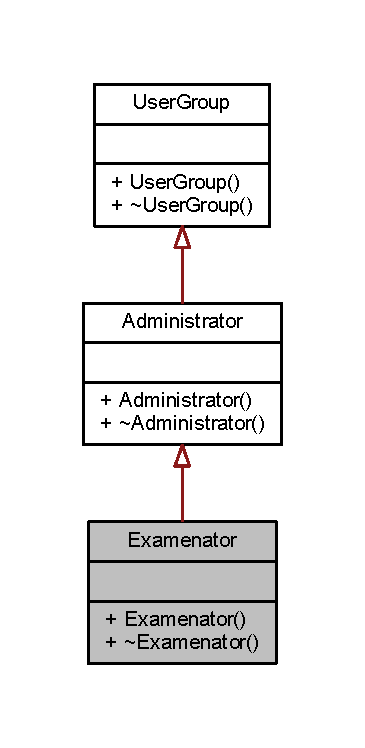
\includegraphics[width=175pt]{d2/db4/class_examenator__inherit__graph}
\end{center}
\end{figure}


Граф связей класса Examenator\+:\nopagebreak
\begin{figure}[H]
\begin{center}
\leavevmode
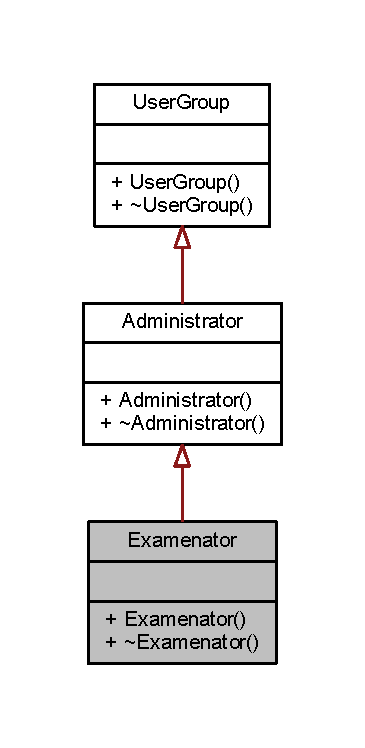
\includegraphics[width=175pt]{dd/d27/class_examenator__coll__graph}
\end{center}
\end{figure}
\subsection*{Открытые члены}
\begin{DoxyCompactItemize}
\item 
\hyperlink{class_examenator_a35ae60e3ea40fed14b1fc2ed72566d43}{Examenator} ()
\item 
\hyperlink{class_examenator_a17573103c56d7f08f1aadf594c1a3f04}{$\sim$\+Examenator} ()
\end{DoxyCompactItemize}
\subsection*{Дополнительные унаследованные члены}


\subsection{Подробное описание}


См. определение в файле Examenator.\+h строка 3



\subsection{Конструктор(ы)}
\hypertarget{class_examenator_a35ae60e3ea40fed14b1fc2ed72566d43}{}\index{Examenator@{Examenator}!Examenator@{Examenator}}
\index{Examenator@{Examenator}!Examenator@{Examenator}}
\subsubsection[{Examenator}]{\setlength{\rightskip}{0pt plus 5cm}Examenator\+::\+Examenator (
\begin{DoxyParamCaption}
{}
\end{DoxyParamCaption}
)}\label{class_examenator_a35ae60e3ea40fed14b1fc2ed72566d43}


См. определение в файле Examenator.\+cpp строка 4

\hypertarget{class_examenator_a17573103c56d7f08f1aadf594c1a3f04}{}\index{Examenator@{Examenator}!````~Examenator@{$\sim$\+Examenator}}
\index{````~Examenator@{$\sim$\+Examenator}!Examenator@{Examenator}}
\subsubsection[{$\sim$\+Examenator}]{\setlength{\rightskip}{0pt plus 5cm}Examenator\+::$\sim$\+Examenator (
\begin{DoxyParamCaption}
{}
\end{DoxyParamCaption}
)}\label{class_examenator_a17573103c56d7f08f1aadf594c1a3f04}


См. определение в файле Examenator.\+cpp строка 9



Объявления и описания членов классов находятся в файлах\+:\begin{DoxyCompactItemize}
\item 
Q\+Tester\+\_\+client/\+Q\+Tester\+\_\+client/\hyperlink{_examenator_8h}{Examenator.\+h}\item 
Q\+Tester\+\_\+client/\+Q\+Tester\+\_\+client/\hyperlink{_examenator_8cpp}{Examenator.\+cpp}\end{DoxyCompactItemize}

\hypertarget{class_examiner}{}\section{Класс Examiner}
\label{class_examiner}\index{Examiner@{Examiner}}


{\ttfamily \#include $<$Examiner.\+h$>$}



Граф наследования\+:Examiner\+:\nopagebreak
\begin{figure}[H]
\begin{center}
\leavevmode
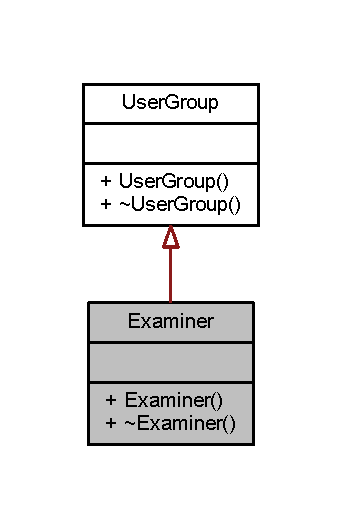
\includegraphics[width=164pt]{d8/dd3/class_examiner__inherit__graph}
\end{center}
\end{figure}


Граф связей класса Examiner\+:\nopagebreak
\begin{figure}[H]
\begin{center}
\leavevmode
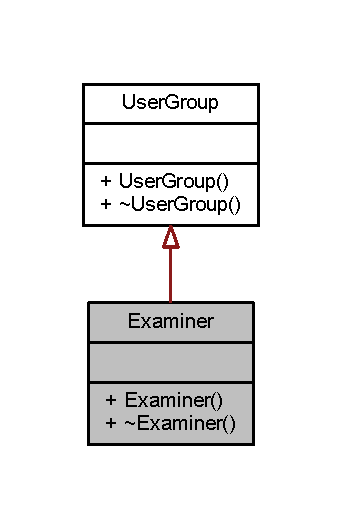
\includegraphics[width=164pt]{d6/d2b/class_examiner__coll__graph}
\end{center}
\end{figure}
\subsection*{Открытые члены}
\begin{DoxyCompactItemize}
\item 
\hyperlink{class_examiner_ac4143d40944e4a18bd480d28edfad8fc}{Examiner} ()
\item 
\hyperlink{class_examiner_a18dfadda51203a4e9de88a288657c2f9}{$\sim$\+Examiner} ()
\end{DoxyCompactItemize}
\subsection*{Дополнительные унаследованные члены}


\subsection{Подробное описание}


См. определение в файле Examiner.\+h строка 3



\subsection{Конструктор(ы)}
\hypertarget{class_examiner_ac4143d40944e4a18bd480d28edfad8fc}{}\index{Examiner@{Examiner}!Examiner@{Examiner}}
\index{Examiner@{Examiner}!Examiner@{Examiner}}
\subsubsection[{Examiner}]{\setlength{\rightskip}{0pt plus 5cm}Examiner\+::\+Examiner (
\begin{DoxyParamCaption}
{}
\end{DoxyParamCaption}
)}\label{class_examiner_ac4143d40944e4a18bd480d28edfad8fc}


См. определение в файле Examiner.\+cpp строка 4

\hypertarget{class_examiner_a18dfadda51203a4e9de88a288657c2f9}{}\index{Examiner@{Examiner}!````~Examiner@{$\sim$\+Examiner}}
\index{````~Examiner@{$\sim$\+Examiner}!Examiner@{Examiner}}
\subsubsection[{$\sim$\+Examiner}]{\setlength{\rightskip}{0pt plus 5cm}Examiner\+::$\sim$\+Examiner (
\begin{DoxyParamCaption}
{}
\end{DoxyParamCaption}
)}\label{class_examiner_a18dfadda51203a4e9de88a288657c2f9}


См. определение в файле Examiner.\+cpp строка 9



Объявления и описания членов классов находятся в файлах\+:\begin{DoxyCompactItemize}
\item 
Q\+Tester\+\_\+client/\+Q\+Tester\+\_\+client/\hyperlink{_examiner_8h}{Examiner.\+h}\item 
Q\+Tester\+\_\+client/\+Q\+Tester\+\_\+client/\hyperlink{_examiner_8cpp}{Examiner.\+cpp}\end{DoxyCompactItemize}

\hypertarget{class_s_q_lite_mgr}{}\section{Класс S\+Q\+Lite\+Mgr}
\label{class_s_q_lite_mgr}\index{S\+Q\+Lite\+Mgr@{S\+Q\+Lite\+Mgr}}


{\ttfamily \#include $<$S\+Q\+Lite\+Mgr.\+h$>$}



Граф наследования\+:S\+Q\+Lite\+Mgr\+:\nopagebreak
\begin{figure}[H]
\begin{center}
\leavevmode
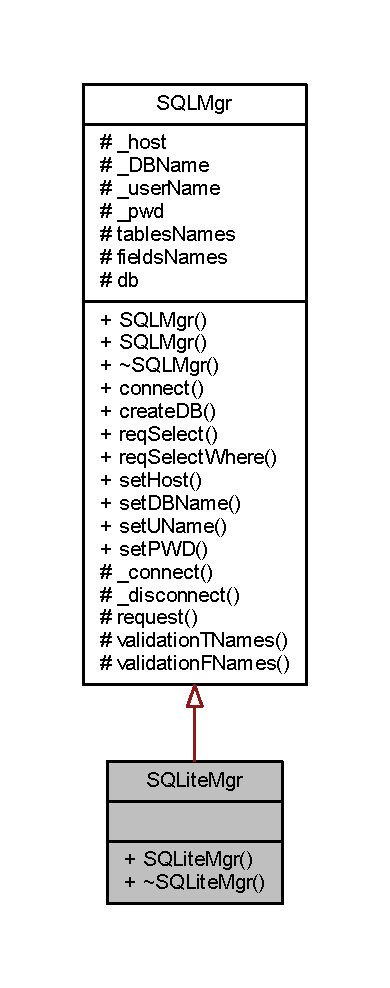
\includegraphics[width=187pt]{d6/d3a/class_s_q_lite_mgr__inherit__graph}
\end{center}
\end{figure}


Граф связей класса S\+Q\+Lite\+Mgr\+:\nopagebreak
\begin{figure}[H]
\begin{center}
\leavevmode
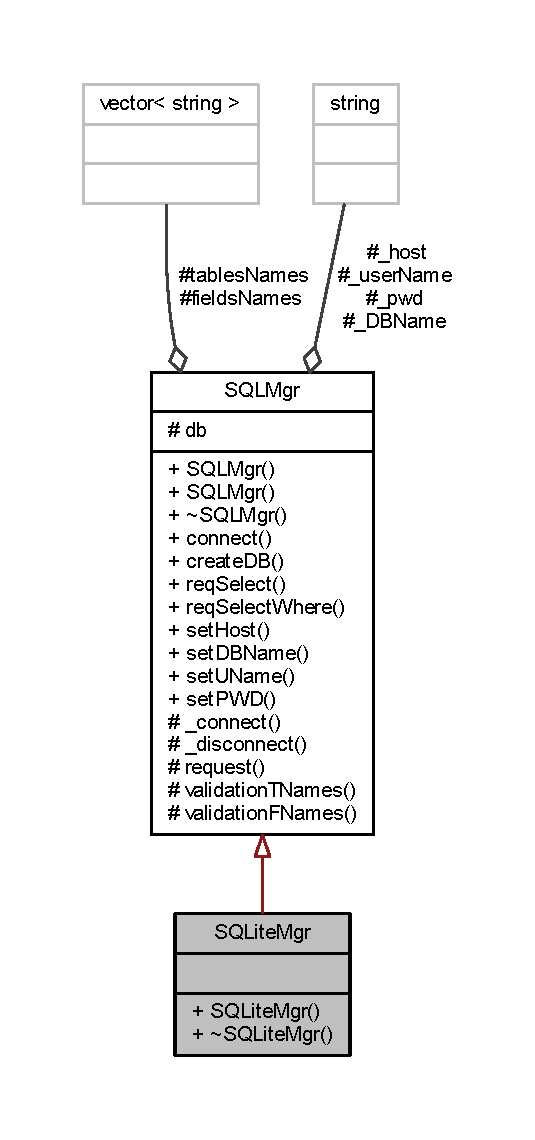
\includegraphics[width=257pt]{d7/deb/class_s_q_lite_mgr__coll__graph}
\end{center}
\end{figure}
\subsection*{Открытые члены}
\begin{DoxyCompactItemize}
\item 
\hyperlink{class_s_q_lite_mgr_a738f1433e21100eb53e262894c6e7095}{S\+Q\+Lite\+Mgr} ()
\item 
\hyperlink{class_s_q_lite_mgr_a341f0009a2d55b8c4642a5fcdce872ea}{$\sim$\+S\+Q\+Lite\+Mgr} ()
\end{DoxyCompactItemize}
\subsection*{Дополнительные унаследованные члены}


\subsection{Подробное описание}


См. определение в файле S\+Q\+Lite\+Mgr.\+h строка 3



\subsection{Конструктор(ы)}
\hypertarget{class_s_q_lite_mgr_a738f1433e21100eb53e262894c6e7095}{}\index{S\+Q\+Lite\+Mgr@{S\+Q\+Lite\+Mgr}!S\+Q\+Lite\+Mgr@{S\+Q\+Lite\+Mgr}}
\index{S\+Q\+Lite\+Mgr@{S\+Q\+Lite\+Mgr}!S\+Q\+Lite\+Mgr@{S\+Q\+Lite\+Mgr}}
\subsubsection[{S\+Q\+Lite\+Mgr}]{\setlength{\rightskip}{0pt plus 5cm}S\+Q\+Lite\+Mgr\+::\+S\+Q\+Lite\+Mgr (
\begin{DoxyParamCaption}
{}
\end{DoxyParamCaption}
)}\label{class_s_q_lite_mgr_a738f1433e21100eb53e262894c6e7095}


См. определение в файле S\+Q\+Lite\+Mgr.\+cpp строка 4

\hypertarget{class_s_q_lite_mgr_a341f0009a2d55b8c4642a5fcdce872ea}{}\index{S\+Q\+Lite\+Mgr@{S\+Q\+Lite\+Mgr}!````~S\+Q\+Lite\+Mgr@{$\sim$\+S\+Q\+Lite\+Mgr}}
\index{````~S\+Q\+Lite\+Mgr@{$\sim$\+S\+Q\+Lite\+Mgr}!S\+Q\+Lite\+Mgr@{S\+Q\+Lite\+Mgr}}
\subsubsection[{$\sim$\+S\+Q\+Lite\+Mgr}]{\setlength{\rightskip}{0pt plus 5cm}S\+Q\+Lite\+Mgr\+::$\sim$\+S\+Q\+Lite\+Mgr (
\begin{DoxyParamCaption}
{}
\end{DoxyParamCaption}
)}\label{class_s_q_lite_mgr_a341f0009a2d55b8c4642a5fcdce872ea}


См. определение в файле S\+Q\+Lite\+Mgr.\+cpp строка 9



Объявления и описания членов классов находятся в файлах\+:\begin{DoxyCompactItemize}
\item 
Q\+Tester\+\_\+client/\+Q\+Tester\+\_\+client/\hyperlink{_s_q_lite_mgr_8h}{S\+Q\+Lite\+Mgr.\+h}\item 
Q\+Tester\+\_\+client/\+Q\+Tester\+\_\+client/\hyperlink{_s_q_lite_mgr_8cpp}{S\+Q\+Lite\+Mgr.\+cpp}\end{DoxyCompactItemize}

\hypertarget{class_s_q_l_mgr}{}\section{Класс S\+Q\+L\+Mgr}
\label{class_s_q_l_mgr}\index{S\+Q\+L\+Mgr@{S\+Q\+L\+Mgr}}


{\ttfamily \#include $<$S\+Q\+L\+Mgr.\+h$>$}



Граф наследования\+:S\+Q\+L\+Mgr\+:\nopagebreak
\begin{figure}[H]
\begin{center}
\leavevmode
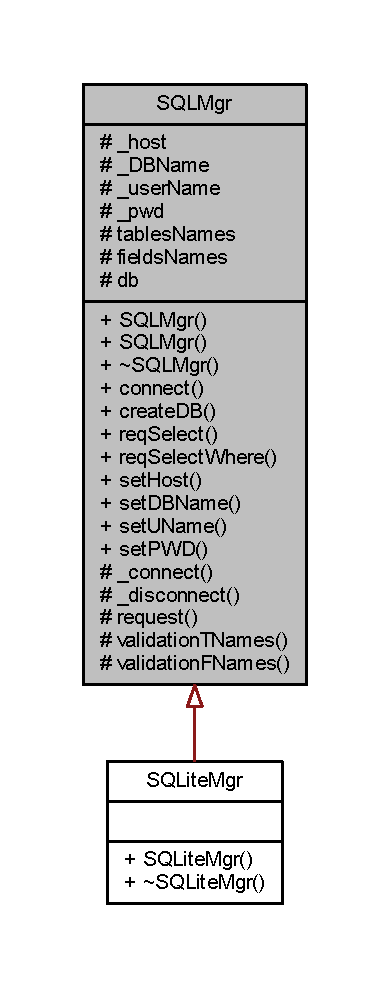
\includegraphics[width=187pt]{df/dc9/class_s_q_l_mgr__inherit__graph}
\end{center}
\end{figure}


Граф связей класса S\+Q\+L\+Mgr\+:\nopagebreak
\begin{figure}[H]
\begin{center}
\leavevmode
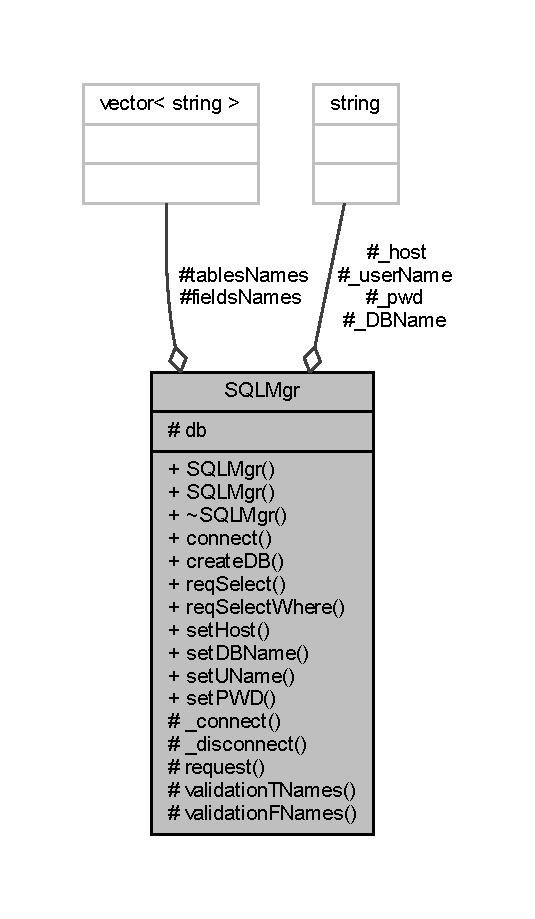
\includegraphics[width=257pt]{d5/dfe/class_s_q_l_mgr__coll__graph}
\end{center}
\end{figure}
\subsection*{Открытые члены}
\begin{DoxyCompactItemize}
\item 
\hyperlink{class_s_q_l_mgr_a9e3713810d0b013ee4637b6381337dca}{S\+Q\+L\+Mgr} ()
\item 
\hyperlink{class_s_q_l_mgr_a5c0e6b8359f138aefaae3c18800bf626}{S\+Q\+L\+Mgr} (string host\+Name, string D\+B\+Name, string user\+Name, string password)
\item 
\hyperlink{class_s_q_l_mgr_a15751c711901e03cf77fc24b37ca492a}{$\sim$\+S\+Q\+L\+Mgr} ()
\item 
void \hyperlink{class_s_q_l_mgr_a8310112b32ccd0913445e31d5cc2fa05}{connect} ()
\item 
void \hyperlink{class_s_q_l_mgr_af272ad3b14f896db101d938009d0b031}{create\+D\+B} ()
\item 
void \hyperlink{class_s_q_l_mgr_a35e46dfc53fdff460b5824a5f679fa5d}{req\+Select} (string fields, string table\+Names)
\item 
void \hyperlink{class_s_q_l_mgr_a823058ef5581b60bb888a58613464630}{req\+Select\+Where} (string fields, string table\+Names, string W\+H\+E\+R\+E)
\item 
void \hyperlink{class_s_q_l_mgr_a62b8a7a6430a4cf193e0ef462e468364}{set\+Host} (string host=\char`\"{}localhost\char`\"{})
\item 
void \hyperlink{class_s_q_l_mgr_ad1770ce2fe7287f0e051fb7deb5c066d}{set\+D\+B\+Name} (string)
\item 
void \hyperlink{class_s_q_l_mgr_adb9f890a6552106c8eb67631fe329c47}{set\+U\+Name} (string)
\item 
void \hyperlink{class_s_q_l_mgr_ad99374f72f5464d5aa8c7e72271282da}{set\+P\+W\+D} (string)
\end{DoxyCompactItemize}
\subsection*{Защищенные члены}
\begin{DoxyCompactItemize}
\item 
virtual void \hyperlink{class_s_q_l_mgr_ac0645ea707c71e5fad141145c1f8b735}{\+\_\+connect} ()
\item 
virtual void \hyperlink{class_s_q_l_mgr_a57da8e9e997d52caa6c4b3051998370d}{\+\_\+disconnect} ()
\item 
virtual bool \hyperlink{class_s_q_l_mgr_af931e8ab90abc8ac125ab7822020167e}{request} (string S\+Q\+L)
\item 
bool \hyperlink{class_s_q_l_mgr_aedb1c3527ed1fb7828eb5a70dda232e1}{validation\+T\+Names} (string T\+Names)
\item 
bool \hyperlink{class_s_q_l_mgr_a7b4d3b9c1526a41c61a91000e17d4dda}{validation\+F\+Names} (string F\+Names)
\end{DoxyCompactItemize}
\subsection*{Защищенные данные}
\begin{DoxyCompactItemize}
\item 
string \hyperlink{class_s_q_l_mgr_ad55ba1fe4d0a5a926575ce4369ec328f}{\+\_\+host}
\item 
string \hyperlink{class_s_q_l_mgr_a73364e875e5b318861734a99a7656966}{\+\_\+\+D\+B\+Name}
\item 
string \hyperlink{class_s_q_l_mgr_a7f66e9b0d44d1e3c988f71dd9a0460df}{\+\_\+user\+Name}
\item 
string \hyperlink{class_s_q_l_mgr_a96279d7c849caa03e154cd777d9c52b9}{\+\_\+pwd}
\item 
vector$<$ string $>$ \hyperlink{class_s_q_l_mgr_ad12619899cd1b12450134f2ecc2ba56c}{tables\+Names}
\item 
vector$<$ string $>$ \hyperlink{class_s_q_l_mgr_a299770e5179d462454a5f343d5b378a2}{fields\+Names}
\item 
Q\+Sql\+Database \hyperlink{class_s_q_l_mgr_a1a950b08b5dc3003ccc164c4f99f5bfd}{db}
\end{DoxyCompactItemize}


\subsection{Подробное описание}


См. определение в файле S\+Q\+L\+Mgr.\+h строка 5



\subsection{Конструктор(ы)}
\hypertarget{class_s_q_l_mgr_a9e3713810d0b013ee4637b6381337dca}{}\index{S\+Q\+L\+Mgr@{S\+Q\+L\+Mgr}!S\+Q\+L\+Mgr@{S\+Q\+L\+Mgr}}
\index{S\+Q\+L\+Mgr@{S\+Q\+L\+Mgr}!S\+Q\+L\+Mgr@{S\+Q\+L\+Mgr}}
\subsubsection[{S\+Q\+L\+Mgr}]{\setlength{\rightskip}{0pt plus 5cm}S\+Q\+L\+Mgr\+::\+S\+Q\+L\+Mgr (
\begin{DoxyParamCaption}
{}
\end{DoxyParamCaption}
)}\label{class_s_q_l_mgr_a9e3713810d0b013ee4637b6381337dca}


См. определение в файле S\+Q\+L\+Mgr.\+cpp строка 4

\hypertarget{class_s_q_l_mgr_a5c0e6b8359f138aefaae3c18800bf626}{}\index{S\+Q\+L\+Mgr@{S\+Q\+L\+Mgr}!S\+Q\+L\+Mgr@{S\+Q\+L\+Mgr}}
\index{S\+Q\+L\+Mgr@{S\+Q\+L\+Mgr}!S\+Q\+L\+Mgr@{S\+Q\+L\+Mgr}}
\subsubsection[{S\+Q\+L\+Mgr}]{\setlength{\rightskip}{0pt plus 5cm}S\+Q\+L\+Mgr\+::\+S\+Q\+L\+Mgr (
\begin{DoxyParamCaption}
\item[{string}]{host\+Name, }
\item[{string}]{D\+B\+Name, }
\item[{string}]{user\+Name, }
\item[{string}]{password}
\end{DoxyParamCaption}
)}\label{class_s_q_l_mgr_a5c0e6b8359f138aefaae3c18800bf626}


См. определение в файле S\+Q\+L\+Mgr.\+cpp строка 8

\hypertarget{class_s_q_l_mgr_a15751c711901e03cf77fc24b37ca492a}{}\index{S\+Q\+L\+Mgr@{S\+Q\+L\+Mgr}!````~S\+Q\+L\+Mgr@{$\sim$\+S\+Q\+L\+Mgr}}
\index{````~S\+Q\+L\+Mgr@{$\sim$\+S\+Q\+L\+Mgr}!S\+Q\+L\+Mgr@{S\+Q\+L\+Mgr}}
\subsubsection[{$\sim$\+S\+Q\+L\+Mgr}]{\setlength{\rightskip}{0pt plus 5cm}S\+Q\+L\+Mgr\+::$\sim$\+S\+Q\+L\+Mgr (
\begin{DoxyParamCaption}
{}
\end{DoxyParamCaption}
)}\label{class_s_q_l_mgr_a15751c711901e03cf77fc24b37ca492a}


См. определение в файле S\+Q\+L\+Mgr.\+cpp строка 14



\subsection{Методы}
\hypertarget{class_s_q_l_mgr_ac0645ea707c71e5fad141145c1f8b735}{}\index{S\+Q\+L\+Mgr@{S\+Q\+L\+Mgr}!\+\_\+connect@{\+\_\+connect}}
\index{\+\_\+connect@{\+\_\+connect}!S\+Q\+L\+Mgr@{S\+Q\+L\+Mgr}}
\subsubsection[{\+\_\+connect}]{\setlength{\rightskip}{0pt plus 5cm}virtual void S\+Q\+L\+Mgr\+::\+\_\+connect (
\begin{DoxyParamCaption}
{}
\end{DoxyParamCaption}
)\hspace{0.3cm}{\ttfamily [protected]}, {\ttfamily [virtual]}}\label{class_s_q_l_mgr_ac0645ea707c71e5fad141145c1f8b735}
\hypertarget{class_s_q_l_mgr_a57da8e9e997d52caa6c4b3051998370d}{}\index{S\+Q\+L\+Mgr@{S\+Q\+L\+Mgr}!\+\_\+disconnect@{\+\_\+disconnect}}
\index{\+\_\+disconnect@{\+\_\+disconnect}!S\+Q\+L\+Mgr@{S\+Q\+L\+Mgr}}
\subsubsection[{\+\_\+disconnect}]{\setlength{\rightskip}{0pt plus 5cm}virtual void S\+Q\+L\+Mgr\+::\+\_\+disconnect (
\begin{DoxyParamCaption}
{}
\end{DoxyParamCaption}
)\hspace{0.3cm}{\ttfamily [protected]}, {\ttfamily [virtual]}}\label{class_s_q_l_mgr_a57da8e9e997d52caa6c4b3051998370d}
\hypertarget{class_s_q_l_mgr_a8310112b32ccd0913445e31d5cc2fa05}{}\index{S\+Q\+L\+Mgr@{S\+Q\+L\+Mgr}!connect@{connect}}
\index{connect@{connect}!S\+Q\+L\+Mgr@{S\+Q\+L\+Mgr}}
\subsubsection[{connect}]{\setlength{\rightskip}{0pt plus 5cm}void S\+Q\+L\+Mgr\+::connect (
\begin{DoxyParamCaption}
{}
\end{DoxyParamCaption}
)}\label{class_s_q_l_mgr_a8310112b32ccd0913445e31d5cc2fa05}
\hypertarget{class_s_q_l_mgr_af272ad3b14f896db101d938009d0b031}{}\index{S\+Q\+L\+Mgr@{S\+Q\+L\+Mgr}!create\+D\+B@{create\+D\+B}}
\index{create\+D\+B@{create\+D\+B}!S\+Q\+L\+Mgr@{S\+Q\+L\+Mgr}}
\subsubsection[{create\+D\+B}]{\setlength{\rightskip}{0pt plus 5cm}void S\+Q\+L\+Mgr\+::create\+D\+B (
\begin{DoxyParamCaption}
{}
\end{DoxyParamCaption}
)}\label{class_s_q_l_mgr_af272ad3b14f896db101d938009d0b031}
\hypertarget{class_s_q_l_mgr_a35e46dfc53fdff460b5824a5f679fa5d}{}\index{S\+Q\+L\+Mgr@{S\+Q\+L\+Mgr}!req\+Select@{req\+Select}}
\index{req\+Select@{req\+Select}!S\+Q\+L\+Mgr@{S\+Q\+L\+Mgr}}
\subsubsection[{req\+Select}]{\setlength{\rightskip}{0pt plus 5cm}void S\+Q\+L\+Mgr\+::req\+Select (
\begin{DoxyParamCaption}
\item[{string}]{fields, }
\item[{string}]{table\+Names}
\end{DoxyParamCaption}
)}\label{class_s_q_l_mgr_a35e46dfc53fdff460b5824a5f679fa5d}
\hypertarget{class_s_q_l_mgr_a823058ef5581b60bb888a58613464630}{}\index{S\+Q\+L\+Mgr@{S\+Q\+L\+Mgr}!req\+Select\+Where@{req\+Select\+Where}}
\index{req\+Select\+Where@{req\+Select\+Where}!S\+Q\+L\+Mgr@{S\+Q\+L\+Mgr}}
\subsubsection[{req\+Select\+Where}]{\setlength{\rightskip}{0pt plus 5cm}void S\+Q\+L\+Mgr\+::req\+Select\+Where (
\begin{DoxyParamCaption}
\item[{string}]{fields, }
\item[{string}]{table\+Names, }
\item[{string}]{W\+H\+E\+R\+E}
\end{DoxyParamCaption}
)}\label{class_s_q_l_mgr_a823058ef5581b60bb888a58613464630}
\hypertarget{class_s_q_l_mgr_af931e8ab90abc8ac125ab7822020167e}{}\index{S\+Q\+L\+Mgr@{S\+Q\+L\+Mgr}!request@{request}}
\index{request@{request}!S\+Q\+L\+Mgr@{S\+Q\+L\+Mgr}}
\subsubsection[{request}]{\setlength{\rightskip}{0pt plus 5cm}virtual bool S\+Q\+L\+Mgr\+::request (
\begin{DoxyParamCaption}
\item[{string}]{S\+Q\+L}
\end{DoxyParamCaption}
)\hspace{0.3cm}{\ttfamily [protected]}, {\ttfamily [virtual]}}\label{class_s_q_l_mgr_af931e8ab90abc8ac125ab7822020167e}
\hypertarget{class_s_q_l_mgr_ad1770ce2fe7287f0e051fb7deb5c066d}{}\index{S\+Q\+L\+Mgr@{S\+Q\+L\+Mgr}!set\+D\+B\+Name@{set\+D\+B\+Name}}
\index{set\+D\+B\+Name@{set\+D\+B\+Name}!S\+Q\+L\+Mgr@{S\+Q\+L\+Mgr}}
\subsubsection[{set\+D\+B\+Name}]{\setlength{\rightskip}{0pt plus 5cm}void S\+Q\+L\+Mgr\+::set\+D\+B\+Name (
\begin{DoxyParamCaption}
\item[{string}]{}
\end{DoxyParamCaption}
)}\label{class_s_q_l_mgr_ad1770ce2fe7287f0e051fb7deb5c066d}
\hypertarget{class_s_q_l_mgr_a62b8a7a6430a4cf193e0ef462e468364}{}\index{S\+Q\+L\+Mgr@{S\+Q\+L\+Mgr}!set\+Host@{set\+Host}}
\index{set\+Host@{set\+Host}!S\+Q\+L\+Mgr@{S\+Q\+L\+Mgr}}
\subsubsection[{set\+Host}]{\setlength{\rightskip}{0pt plus 5cm}void S\+Q\+L\+Mgr\+::set\+Host (
\begin{DoxyParamCaption}
\item[{string}]{host = {\ttfamily \char`\"{}localhost\char`\"{}}}
\end{DoxyParamCaption}
)}\label{class_s_q_l_mgr_a62b8a7a6430a4cf193e0ef462e468364}
\hypertarget{class_s_q_l_mgr_ad99374f72f5464d5aa8c7e72271282da}{}\index{S\+Q\+L\+Mgr@{S\+Q\+L\+Mgr}!set\+P\+W\+D@{set\+P\+W\+D}}
\index{set\+P\+W\+D@{set\+P\+W\+D}!S\+Q\+L\+Mgr@{S\+Q\+L\+Mgr}}
\subsubsection[{set\+P\+W\+D}]{\setlength{\rightskip}{0pt plus 5cm}void S\+Q\+L\+Mgr\+::set\+P\+W\+D (
\begin{DoxyParamCaption}
\item[{string}]{}
\end{DoxyParamCaption}
)}\label{class_s_q_l_mgr_ad99374f72f5464d5aa8c7e72271282da}
\hypertarget{class_s_q_l_mgr_adb9f890a6552106c8eb67631fe329c47}{}\index{S\+Q\+L\+Mgr@{S\+Q\+L\+Mgr}!set\+U\+Name@{set\+U\+Name}}
\index{set\+U\+Name@{set\+U\+Name}!S\+Q\+L\+Mgr@{S\+Q\+L\+Mgr}}
\subsubsection[{set\+U\+Name}]{\setlength{\rightskip}{0pt plus 5cm}void S\+Q\+L\+Mgr\+::set\+U\+Name (
\begin{DoxyParamCaption}
\item[{string}]{}
\end{DoxyParamCaption}
)}\label{class_s_q_l_mgr_adb9f890a6552106c8eb67631fe329c47}
\hypertarget{class_s_q_l_mgr_a7b4d3b9c1526a41c61a91000e17d4dda}{}\index{S\+Q\+L\+Mgr@{S\+Q\+L\+Mgr}!validation\+F\+Names@{validation\+F\+Names}}
\index{validation\+F\+Names@{validation\+F\+Names}!S\+Q\+L\+Mgr@{S\+Q\+L\+Mgr}}
\subsubsection[{validation\+F\+Names}]{\setlength{\rightskip}{0pt plus 5cm}bool S\+Q\+L\+Mgr\+::validation\+F\+Names (
\begin{DoxyParamCaption}
\item[{string}]{F\+Names}
\end{DoxyParamCaption}
)\hspace{0.3cm}{\ttfamily [protected]}}\label{class_s_q_l_mgr_a7b4d3b9c1526a41c61a91000e17d4dda}
\hypertarget{class_s_q_l_mgr_aedb1c3527ed1fb7828eb5a70dda232e1}{}\index{S\+Q\+L\+Mgr@{S\+Q\+L\+Mgr}!validation\+T\+Names@{validation\+T\+Names}}
\index{validation\+T\+Names@{validation\+T\+Names}!S\+Q\+L\+Mgr@{S\+Q\+L\+Mgr}}
\subsubsection[{validation\+T\+Names}]{\setlength{\rightskip}{0pt plus 5cm}bool S\+Q\+L\+Mgr\+::validation\+T\+Names (
\begin{DoxyParamCaption}
\item[{string}]{T\+Names}
\end{DoxyParamCaption}
)\hspace{0.3cm}{\ttfamily [protected]}}\label{class_s_q_l_mgr_aedb1c3527ed1fb7828eb5a70dda232e1}


\subsection{Данные класса}
\hypertarget{class_s_q_l_mgr_a73364e875e5b318861734a99a7656966}{}\index{S\+Q\+L\+Mgr@{S\+Q\+L\+Mgr}!\+\_\+\+D\+B\+Name@{\+\_\+\+D\+B\+Name}}
\index{\+\_\+\+D\+B\+Name@{\+\_\+\+D\+B\+Name}!S\+Q\+L\+Mgr@{S\+Q\+L\+Mgr}}
\subsubsection[{\+\_\+\+D\+B\+Name}]{\setlength{\rightskip}{0pt plus 5cm}string S\+Q\+L\+Mgr\+::\+\_\+\+D\+B\+Name\hspace{0.3cm}{\ttfamily [protected]}}\label{class_s_q_l_mgr_a73364e875e5b318861734a99a7656966}


См. определение в файле S\+Q\+L\+Mgr.\+h строка 10

\hypertarget{class_s_q_l_mgr_ad55ba1fe4d0a5a926575ce4369ec328f}{}\index{S\+Q\+L\+Mgr@{S\+Q\+L\+Mgr}!\+\_\+host@{\+\_\+host}}
\index{\+\_\+host@{\+\_\+host}!S\+Q\+L\+Mgr@{S\+Q\+L\+Mgr}}
\subsubsection[{\+\_\+host}]{\setlength{\rightskip}{0pt plus 5cm}string S\+Q\+L\+Mgr\+::\+\_\+host\hspace{0.3cm}{\ttfamily [protected]}}\label{class_s_q_l_mgr_ad55ba1fe4d0a5a926575ce4369ec328f}


См. определение в файле S\+Q\+L\+Mgr.\+h строка 9

\hypertarget{class_s_q_l_mgr_a96279d7c849caa03e154cd777d9c52b9}{}\index{S\+Q\+L\+Mgr@{S\+Q\+L\+Mgr}!\+\_\+pwd@{\+\_\+pwd}}
\index{\+\_\+pwd@{\+\_\+pwd}!S\+Q\+L\+Mgr@{S\+Q\+L\+Mgr}}
\subsubsection[{\+\_\+pwd}]{\setlength{\rightskip}{0pt plus 5cm}string S\+Q\+L\+Mgr\+::\+\_\+pwd\hspace{0.3cm}{\ttfamily [protected]}}\label{class_s_q_l_mgr_a96279d7c849caa03e154cd777d9c52b9}


См. определение в файле S\+Q\+L\+Mgr.\+h строка 12

\hypertarget{class_s_q_l_mgr_a7f66e9b0d44d1e3c988f71dd9a0460df}{}\index{S\+Q\+L\+Mgr@{S\+Q\+L\+Mgr}!\+\_\+user\+Name@{\+\_\+user\+Name}}
\index{\+\_\+user\+Name@{\+\_\+user\+Name}!S\+Q\+L\+Mgr@{S\+Q\+L\+Mgr}}
\subsubsection[{\+\_\+user\+Name}]{\setlength{\rightskip}{0pt plus 5cm}string S\+Q\+L\+Mgr\+::\+\_\+user\+Name\hspace{0.3cm}{\ttfamily [protected]}}\label{class_s_q_l_mgr_a7f66e9b0d44d1e3c988f71dd9a0460df}


См. определение в файле S\+Q\+L\+Mgr.\+h строка 11

\hypertarget{class_s_q_l_mgr_a1a950b08b5dc3003ccc164c4f99f5bfd}{}\index{S\+Q\+L\+Mgr@{S\+Q\+L\+Mgr}!db@{db}}
\index{db@{db}!S\+Q\+L\+Mgr@{S\+Q\+L\+Mgr}}
\subsubsection[{db}]{\setlength{\rightskip}{0pt plus 5cm}Q\+Sql\+Database S\+Q\+L\+Mgr\+::db\hspace{0.3cm}{\ttfamily [protected]}}\label{class_s_q_l_mgr_a1a950b08b5dc3003ccc164c4f99f5bfd}


См. определение в файле S\+Q\+L\+Mgr.\+h строка 16

\hypertarget{class_s_q_l_mgr_a299770e5179d462454a5f343d5b378a2}{}\index{S\+Q\+L\+Mgr@{S\+Q\+L\+Mgr}!fields\+Names@{fields\+Names}}
\index{fields\+Names@{fields\+Names}!S\+Q\+L\+Mgr@{S\+Q\+L\+Mgr}}
\subsubsection[{fields\+Names}]{\setlength{\rightskip}{0pt plus 5cm}vector$<$string$>$ S\+Q\+L\+Mgr\+::fields\+Names\hspace{0.3cm}{\ttfamily [protected]}}\label{class_s_q_l_mgr_a299770e5179d462454a5f343d5b378a2}


См. определение в файле S\+Q\+L\+Mgr.\+h строка 15

\hypertarget{class_s_q_l_mgr_ad12619899cd1b12450134f2ecc2ba56c}{}\index{S\+Q\+L\+Mgr@{S\+Q\+L\+Mgr}!tables\+Names@{tables\+Names}}
\index{tables\+Names@{tables\+Names}!S\+Q\+L\+Mgr@{S\+Q\+L\+Mgr}}
\subsubsection[{tables\+Names}]{\setlength{\rightskip}{0pt plus 5cm}vector$<$string$>$ S\+Q\+L\+Mgr\+::tables\+Names\hspace{0.3cm}{\ttfamily [protected]}}\label{class_s_q_l_mgr_ad12619899cd1b12450134f2ecc2ba56c}


См. определение в файле S\+Q\+L\+Mgr.\+h строка 14



Объявления и описания членов классов находятся в файлах\+:\begin{DoxyCompactItemize}
\item 
Q\+Tester\+\_\+client/\+Q\+Tester\+\_\+client/\hyperlink{_s_q_l_mgr_8h}{S\+Q\+L\+Mgr.\+h}\item 
Q\+Tester\+\_\+client/\+Q\+Tester\+\_\+client/\hyperlink{_s_q_l_mgr_8cpp}{S\+Q\+L\+Mgr.\+cpp}\end{DoxyCompactItemize}

\hypertarget{class_student}{}\section{Класс Student}
\label{class_student}\index{Student@{Student}}


{\ttfamily \#include $<$Student.\+h$>$}



Граф наследования\+:Student\+:\nopagebreak
\begin{figure}[H]
\begin{center}
\leavevmode
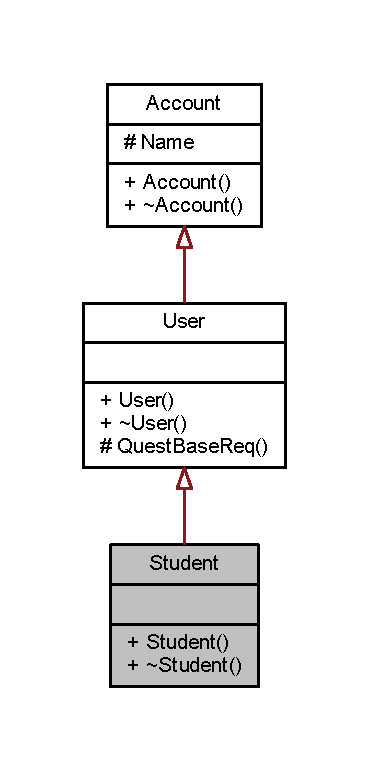
\includegraphics[width=177pt]{d1/d6b/class_student__inherit__graph}
\end{center}
\end{figure}


Граф связей класса Student\+:\nopagebreak
\begin{figure}[H]
\begin{center}
\leavevmode
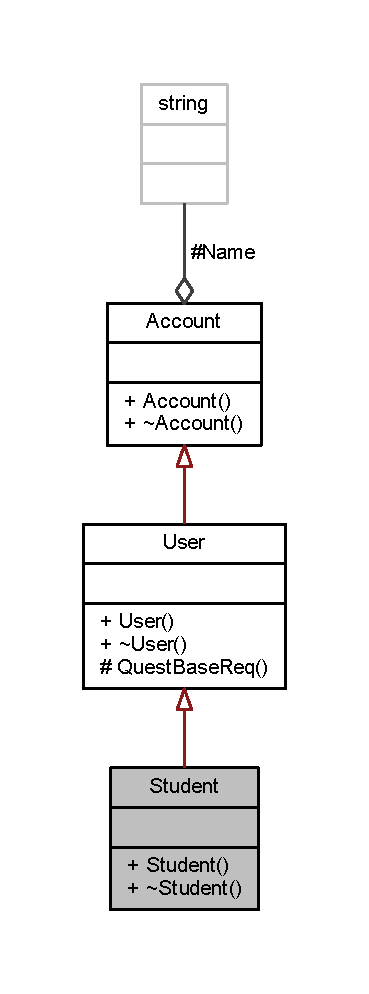
\includegraphics[width=177pt]{dd/db9/class_student__coll__graph}
\end{center}
\end{figure}
\subsection*{Открытые члены}
\begin{DoxyCompactItemize}
\item 
\hyperlink{class_student_af9168cedbfa5565cf0b20c1a9d3f5c9d}{Student} ()
\item 
\hyperlink{class_student_a54a8ea060d6cd04222c3a2f89829f105}{$\sim$\+Student} ()
\end{DoxyCompactItemize}
\subsection*{Дополнительные унаследованные члены}


\subsection{Подробное описание}


См. определение в файле Student.\+h строка 3



\subsection{Конструктор(ы)}
\hypertarget{class_student_af9168cedbfa5565cf0b20c1a9d3f5c9d}{}\index{Student@{Student}!Student@{Student}}
\index{Student@{Student}!Student@{Student}}
\subsubsection[{Student}]{\setlength{\rightskip}{0pt plus 5cm}Student\+::\+Student (
\begin{DoxyParamCaption}
{}
\end{DoxyParamCaption}
)}\label{class_student_af9168cedbfa5565cf0b20c1a9d3f5c9d}


См. определение в файле Student.\+cpp строка 3

\hypertarget{class_student_a54a8ea060d6cd04222c3a2f89829f105}{}\index{Student@{Student}!````~Student@{$\sim$\+Student}}
\index{````~Student@{$\sim$\+Student}!Student@{Student}}
\subsubsection[{$\sim$\+Student}]{\setlength{\rightskip}{0pt plus 5cm}Student\+::$\sim$\+Student (
\begin{DoxyParamCaption}
{}
\end{DoxyParamCaption}
)}\label{class_student_a54a8ea060d6cd04222c3a2f89829f105}


См. определение в файле Student.\+cpp строка 8



Объявления и описания членов классов находятся в файлах\+:\begin{DoxyCompactItemize}
\item 
Q\+Tester\+\_\+client/\+Q\+Tester\+\_\+client/\hyperlink{_student_8h}{Student.\+h}\item 
Q\+Tester\+\_\+client/\+Q\+Tester\+\_\+client/\hyperlink{_student_8cpp}{Student.\+cpp}\end{DoxyCompactItemize}

\hypertarget{class_teacher}{}\section{Класс Teacher}
\label{class_teacher}\index{Teacher@{Teacher}}


{\ttfamily \#include $<$Teacher.\+h$>$}



Граф наследования\+:Teacher\+:\nopagebreak
\begin{figure}[H]
\begin{center}
\leavevmode
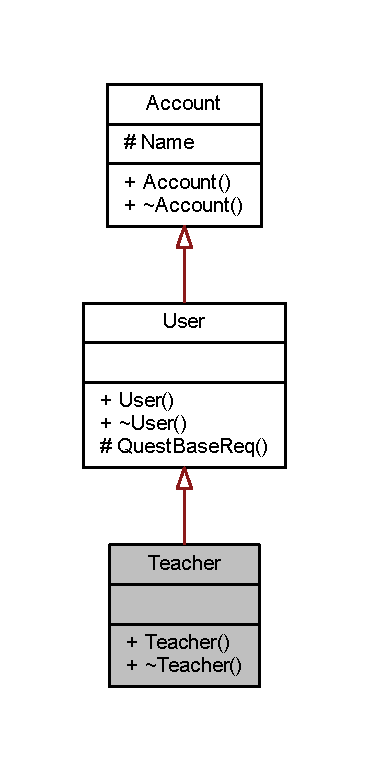
\includegraphics[width=177pt]{d7/d13/class_teacher__inherit__graph}
\end{center}
\end{figure}


Граф связей класса Teacher\+:\nopagebreak
\begin{figure}[H]
\begin{center}
\leavevmode
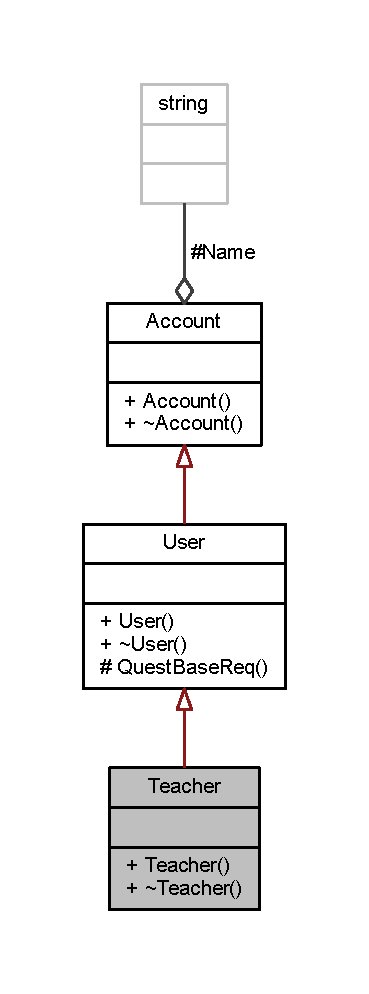
\includegraphics[width=177pt]{d0/dbe/class_teacher__coll__graph}
\end{center}
\end{figure}
\subsection*{Открытые члены}
\begin{DoxyCompactItemize}
\item 
\hyperlink{class_teacher_a0d09b151c46e2abb647a2ae40cc5510c}{Teacher} ()
\item 
\hyperlink{class_teacher_a27e515506e87deffe0cb21e26c4df90c}{$\sim$\+Teacher} ()
\end{DoxyCompactItemize}
\subsection*{Дополнительные унаследованные члены}


\subsection{Подробное описание}


См. определение в файле Teacher.\+h строка 3



\subsection{Конструктор(ы)}
\hypertarget{class_teacher_a0d09b151c46e2abb647a2ae40cc5510c}{}\index{Teacher@{Teacher}!Teacher@{Teacher}}
\index{Teacher@{Teacher}!Teacher@{Teacher}}
\subsubsection[{Teacher}]{\setlength{\rightskip}{0pt plus 5cm}Teacher\+::\+Teacher (
\begin{DoxyParamCaption}
{}
\end{DoxyParamCaption}
)}\label{class_teacher_a0d09b151c46e2abb647a2ae40cc5510c}


См. определение в файле Teacher.\+cpp строка 4

\hypertarget{class_teacher_a27e515506e87deffe0cb21e26c4df90c}{}\index{Teacher@{Teacher}!````~Teacher@{$\sim$\+Teacher}}
\index{````~Teacher@{$\sim$\+Teacher}!Teacher@{Teacher}}
\subsubsection[{$\sim$\+Teacher}]{\setlength{\rightskip}{0pt plus 5cm}Teacher\+::$\sim$\+Teacher (
\begin{DoxyParamCaption}
{}
\end{DoxyParamCaption}
)}\label{class_teacher_a27e515506e87deffe0cb21e26c4df90c}


См. определение в файле Teacher.\+cpp строка 9



Объявления и описания членов классов находятся в файлах\+:\begin{DoxyCompactItemize}
\item 
Q\+Tester\+\_\+client/\+Q\+Tester\+\_\+client/\hyperlink{_teacher_8h}{Teacher.\+h}\item 
Q\+Tester\+\_\+client/\+Q\+Tester\+\_\+client/\hyperlink{_teacher_8cpp}{Teacher.\+cpp}\end{DoxyCompactItemize}

\hypertarget{class_tester}{}\section{Класс Tester}
\label{class_tester}\index{Tester@{Tester}}


{\ttfamily \#include $<$Tester.\+h$>$}



Граф связей класса Tester\+:\nopagebreak
\begin{figure}[H]
\begin{center}
\leavevmode
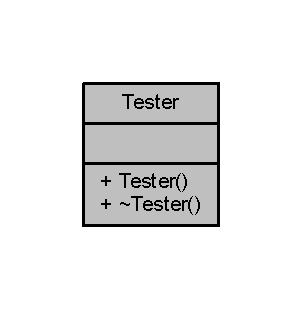
\includegraphics[width=145pt]{dd/d61/class_tester__coll__graph}
\end{center}
\end{figure}
\subsection*{Открытые члены}
\begin{DoxyCompactItemize}
\item 
\hyperlink{class_tester_ad70b2b2bbf6c564e710680ec1e0ae2d6}{Tester} ()
\item 
\hyperlink{class_tester_afbbc09a4e930a03889711ff79ee6cfb0}{$\sim$\+Tester} ()
\end{DoxyCompactItemize}


\subsection{Подробное описание}


См. определение в файле Tester.\+h строка 2



\subsection{Конструктор(ы)}
\hypertarget{class_tester_ad70b2b2bbf6c564e710680ec1e0ae2d6}{}\index{Tester@{Tester}!Tester@{Tester}}
\index{Tester@{Tester}!Tester@{Tester}}
\subsubsection[{Tester}]{\setlength{\rightskip}{0pt plus 5cm}Tester\+::\+Tester (
\begin{DoxyParamCaption}
{}
\end{DoxyParamCaption}
)}\label{class_tester_ad70b2b2bbf6c564e710680ec1e0ae2d6}


См. определение в файле Tester.\+cpp строка 4

\hypertarget{class_tester_afbbc09a4e930a03889711ff79ee6cfb0}{}\index{Tester@{Tester}!````~Tester@{$\sim$\+Tester}}
\index{````~Tester@{$\sim$\+Tester}!Tester@{Tester}}
\subsubsection[{$\sim$\+Tester}]{\setlength{\rightskip}{0pt plus 5cm}Tester\+::$\sim$\+Tester (
\begin{DoxyParamCaption}
{}
\end{DoxyParamCaption}
)}\label{class_tester_afbbc09a4e930a03889711ff79ee6cfb0}


См. определение в файле Tester.\+cpp строка 9



Объявления и описания членов классов находятся в файлах\+:\begin{DoxyCompactItemize}
\item 
Q\+Tester\+\_\+client/\+Q\+Tester\+\_\+client/\hyperlink{_tester_8h}{Tester.\+h}\item 
Q\+Tester\+\_\+client/\+Q\+Tester\+\_\+client/\hyperlink{_tester_8cpp}{Tester.\+cpp}\end{DoxyCompactItemize}

\hypertarget{class_test_generator}{}\section{Класс Test\+Generator}
\label{class_test_generator}\index{Test\+Generator@{Test\+Generator}}


{\ttfamily \#include $<$Test\+Generator.\+h$>$}



Граф связей класса Test\+Generator\+:\nopagebreak
\begin{figure}[H]
\begin{center}
\leavevmode
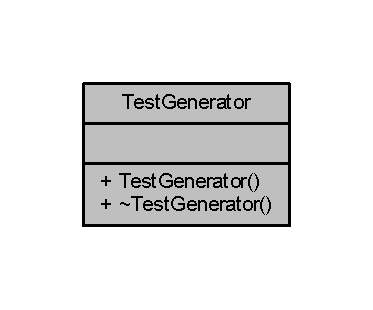
\includegraphics[width=179pt]{db/d6b/class_test_generator__coll__graph}
\end{center}
\end{figure}
\subsection*{Открытые члены}
\begin{DoxyCompactItemize}
\item 
\hyperlink{class_test_generator_abf2f8f12559efb7d8a59e761dcb5f5bf}{Test\+Generator} ()
\item 
\hyperlink{class_test_generator_ac995d1016cf9df7c8caf0c014af5cd33}{$\sim$\+Test\+Generator} ()
\end{DoxyCompactItemize}


\subsection{Подробное описание}


См. определение в файле Test\+Generator.\+h строка 2



\subsection{Конструктор(ы)}
\hypertarget{class_test_generator_abf2f8f12559efb7d8a59e761dcb5f5bf}{}\index{Test\+Generator@{Test\+Generator}!Test\+Generator@{Test\+Generator}}
\index{Test\+Generator@{Test\+Generator}!Test\+Generator@{Test\+Generator}}
\subsubsection[{Test\+Generator}]{\setlength{\rightskip}{0pt plus 5cm}Test\+Generator\+::\+Test\+Generator (
\begin{DoxyParamCaption}
{}
\end{DoxyParamCaption}
)}\label{class_test_generator_abf2f8f12559efb7d8a59e761dcb5f5bf}


См. определение в файле Test\+Generator.\+cpp строка 4

\hypertarget{class_test_generator_ac995d1016cf9df7c8caf0c014af5cd33}{}\index{Test\+Generator@{Test\+Generator}!````~Test\+Generator@{$\sim$\+Test\+Generator}}
\index{````~Test\+Generator@{$\sim$\+Test\+Generator}!Test\+Generator@{Test\+Generator}}
\subsubsection[{$\sim$\+Test\+Generator}]{\setlength{\rightskip}{0pt plus 5cm}Test\+Generator\+::$\sim$\+Test\+Generator (
\begin{DoxyParamCaption}
{}
\end{DoxyParamCaption}
)}\label{class_test_generator_ac995d1016cf9df7c8caf0c014af5cd33}


См. определение в файле Test\+Generator.\+cpp строка 9



Объявления и описания членов классов находятся в файлах\+:\begin{DoxyCompactItemize}
\item 
Q\+Tester\+\_\+client/\+Q\+Tester\+\_\+client/\hyperlink{_test_generator_8h}{Test\+Generator.\+h}\item 
Q\+Tester\+\_\+client/\+Q\+Tester\+\_\+client/\hyperlink{_test_generator_8cpp}{Test\+Generator.\+cpp}\end{DoxyCompactItemize}

\hypertarget{class_u_a_c}{}\section{Класс U\+A\+C}
\label{class_u_a_c}\index{U\+A\+C@{U\+A\+C}}


{\ttfamily \#include $<$U\+A\+C.\+h$>$}



Граф связей класса U\+A\+C\+:\nopagebreak
\begin{figure}[H]
\begin{center}
\leavevmode
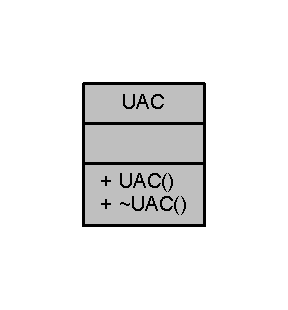
\includegraphics[width=138pt]{dc/db6/class_u_a_c__coll__graph}
\end{center}
\end{figure}
\subsection*{Открытые члены}
\begin{DoxyCompactItemize}
\item 
\hyperlink{class_u_a_c_a6b071a5eaa3f578566476be493118a94}{U\+A\+C} ()
\item 
\hyperlink{class_u_a_c_abbe76cf5f9ad3a12530b13adaf8eed1d}{$\sim$\+U\+A\+C} ()
\end{DoxyCompactItemize}


\subsection{Подробное описание}


См. определение в файле U\+A\+C.\+h строка 4



\subsection{Конструктор(ы)}
\hypertarget{class_u_a_c_a6b071a5eaa3f578566476be493118a94}{}\index{U\+A\+C@{U\+A\+C}!U\+A\+C@{U\+A\+C}}
\index{U\+A\+C@{U\+A\+C}!U\+A\+C@{U\+A\+C}}
\subsubsection[{U\+A\+C}]{\setlength{\rightskip}{0pt plus 5cm}U\+A\+C\+::\+U\+A\+C (
\begin{DoxyParamCaption}
{}
\end{DoxyParamCaption}
)}\label{class_u_a_c_a6b071a5eaa3f578566476be493118a94}


См. определение в файле U\+A\+C.\+cpp строка 4

\hypertarget{class_u_a_c_abbe76cf5f9ad3a12530b13adaf8eed1d}{}\index{U\+A\+C@{U\+A\+C}!````~U\+A\+C@{$\sim$\+U\+A\+C}}
\index{````~U\+A\+C@{$\sim$\+U\+A\+C}!U\+A\+C@{U\+A\+C}}
\subsubsection[{$\sim$\+U\+A\+C}]{\setlength{\rightskip}{0pt plus 5cm}U\+A\+C\+::$\sim$\+U\+A\+C (
\begin{DoxyParamCaption}
{}
\end{DoxyParamCaption}
)}\label{class_u_a_c_abbe76cf5f9ad3a12530b13adaf8eed1d}


См. определение в файле U\+A\+C.\+cpp строка 9



Объявления и описания членов классов находятся в файлах\+:\begin{DoxyCompactItemize}
\item 
Q\+Tester\+\_\+client/\+Q\+Tester\+\_\+client/\hyperlink{_u_a_c_8h}{U\+A\+C.\+h}\item 
Q\+Tester\+\_\+client/\+Q\+Tester\+\_\+client/\hyperlink{_u_a_c_8cpp}{U\+A\+C.\+cpp}\end{DoxyCompactItemize}

\hypertarget{class_user}{}\section{Класс User}
\label{class_user}\index{User@{User}}


{\ttfamily \#include $<$User.\+h$>$}



Граф наследования\+:User\+:\nopagebreak
\begin{figure}[H]
\begin{center}
\leavevmode
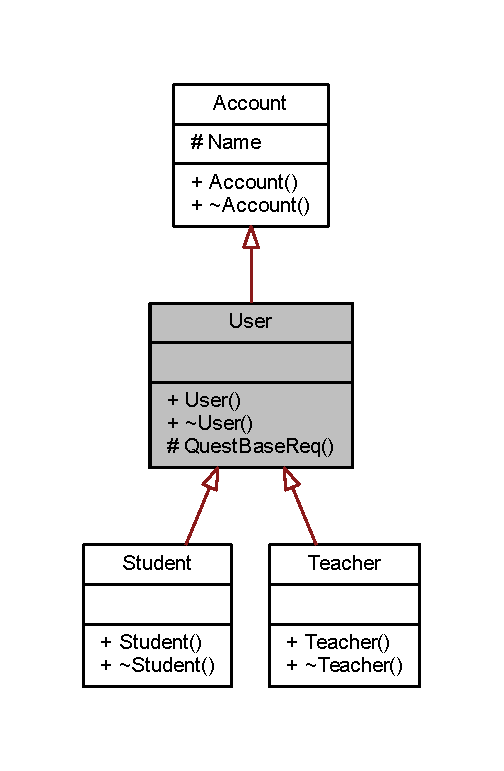
\includegraphics[width=242pt]{d4/dbc/class_user__inherit__graph}
\end{center}
\end{figure}


Граф связей класса User\+:\nopagebreak
\begin{figure}[H]
\begin{center}
\leavevmode
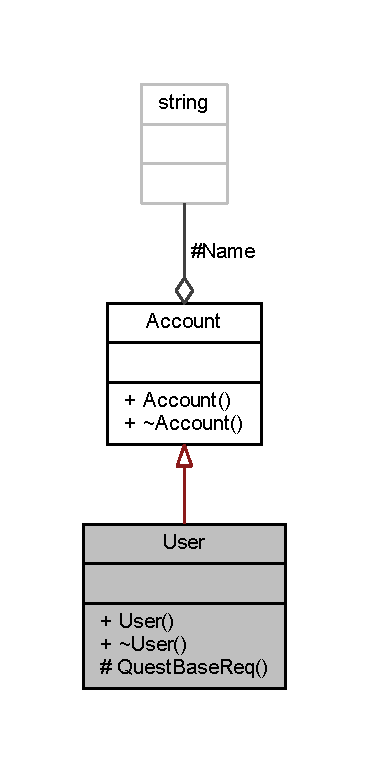
\includegraphics[width=177pt]{d6/d8a/class_user__coll__graph}
\end{center}
\end{figure}
\subsection*{Открытые члены}
\begin{DoxyCompactItemize}
\item 
\hyperlink{class_user_a4a0137053e591fbb79d9057dd7d2283d}{User} ()
\item 
\hyperlink{class_user_ac00b72ad64eb4149f7b21b9f5468c2b2}{$\sim$\+User} ()
\end{DoxyCompactItemize}
\subsection*{Защищенные члены}
\begin{DoxyCompactItemize}
\item 
virtual void \hyperlink{class_user_acadb47688ed7480653f51686380425bb}{Quest\+Base\+Req} ()
\end{DoxyCompactItemize}
\subsection*{Дополнительные унаследованные члены}


\subsection{Подробное описание}


См. определение в файле User.\+h строка 4



\subsection{Конструктор(ы)}
\hypertarget{class_user_a4a0137053e591fbb79d9057dd7d2283d}{}\index{User@{User}!User@{User}}
\index{User@{User}!User@{User}}
\subsubsection[{User}]{\setlength{\rightskip}{0pt plus 5cm}User\+::\+User (
\begin{DoxyParamCaption}
{}
\end{DoxyParamCaption}
)}\label{class_user_a4a0137053e591fbb79d9057dd7d2283d}


См. определение в файле User.\+cpp строка 4

\hypertarget{class_user_ac00b72ad64eb4149f7b21b9f5468c2b2}{}\index{User@{User}!````~User@{$\sim$\+User}}
\index{````~User@{$\sim$\+User}!User@{User}}
\subsubsection[{$\sim$\+User}]{\setlength{\rightskip}{0pt plus 5cm}User\+::$\sim$\+User (
\begin{DoxyParamCaption}
{}
\end{DoxyParamCaption}
)}\label{class_user_ac00b72ad64eb4149f7b21b9f5468c2b2}


См. определение в файле User.\+cpp строка 9



\subsection{Методы}
\hypertarget{class_user_acadb47688ed7480653f51686380425bb}{}\index{User@{User}!Quest\+Base\+Req@{Quest\+Base\+Req}}
\index{Quest\+Base\+Req@{Quest\+Base\+Req}!User@{User}}
\subsubsection[{Quest\+Base\+Req}]{\setlength{\rightskip}{0pt plus 5cm}virtual void User\+::\+Quest\+Base\+Req (
\begin{DoxyParamCaption}
{}
\end{DoxyParamCaption}
)\hspace{0.3cm}{\ttfamily [protected]}, {\ttfamily [virtual]}}\label{class_user_acadb47688ed7480653f51686380425bb}


Объявления и описания членов классов находятся в файлах\+:\begin{DoxyCompactItemize}
\item 
Q\+Tester\+\_\+client/\+Q\+Tester\+\_\+client/\hyperlink{_user_8h}{User.\+h}\item 
Q\+Tester\+\_\+client/\+Q\+Tester\+\_\+client/\hyperlink{_user_8cpp}{User.\+cpp}\end{DoxyCompactItemize}

\hypertarget{class_user_group}{}\section{Класс User\+Group}
\label{class_user_group}\index{User\+Group@{User\+Group}}


{\ttfamily \#include $<$User\+Group.\+h$>$}



Граф наследования\+:User\+Group\+:\nopagebreak
\begin{figure}[H]
\begin{center}
\leavevmode
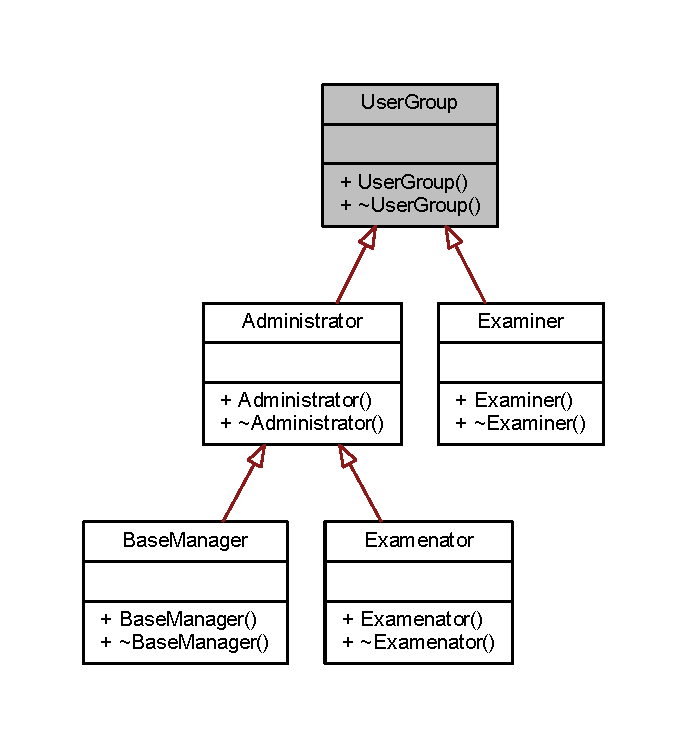
\includegraphics[width=330pt]{d3/dd2/class_user_group__inherit__graph}
\end{center}
\end{figure}


Граф связей класса User\+Group\+:\nopagebreak
\begin{figure}[H]
\begin{center}
\leavevmode
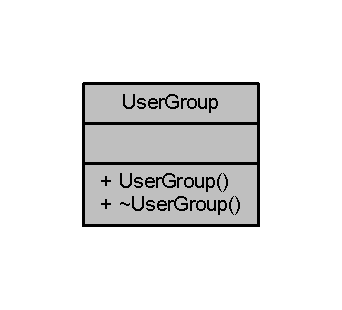
\includegraphics[width=164pt]{df/dd4/class_user_group__coll__graph}
\end{center}
\end{figure}
\subsection*{Открытые члены}
\begin{DoxyCompactItemize}
\item 
\hyperlink{class_user_group_acea0799d207b9f21c9d5cd67278ba528}{User\+Group} ()
\item 
\hyperlink{class_user_group_a5ec79eb4570643e71e5baf871417dae2}{$\sim$\+User\+Group} ()
\end{DoxyCompactItemize}


\subsection{Подробное описание}


См. определение в файле User\+Group.\+h строка 2



\subsection{Конструктор(ы)}
\hypertarget{class_user_group_acea0799d207b9f21c9d5cd67278ba528}{}\index{User\+Group@{User\+Group}!User\+Group@{User\+Group}}
\index{User\+Group@{User\+Group}!User\+Group@{User\+Group}}
\subsubsection[{User\+Group}]{\setlength{\rightskip}{0pt plus 5cm}User\+Group\+::\+User\+Group (
\begin{DoxyParamCaption}
{}
\end{DoxyParamCaption}
)}\label{class_user_group_acea0799d207b9f21c9d5cd67278ba528}


См. определение в файле User\+Group.\+cpp строка 4

\hypertarget{class_user_group_a5ec79eb4570643e71e5baf871417dae2}{}\index{User\+Group@{User\+Group}!````~User\+Group@{$\sim$\+User\+Group}}
\index{````~User\+Group@{$\sim$\+User\+Group}!User\+Group@{User\+Group}}
\subsubsection[{$\sim$\+User\+Group}]{\setlength{\rightskip}{0pt plus 5cm}User\+Group\+::$\sim$\+User\+Group (
\begin{DoxyParamCaption}
{}
\end{DoxyParamCaption}
)}\label{class_user_group_a5ec79eb4570643e71e5baf871417dae2}


См. определение в файле User\+Group.\+cpp строка 9



Объявления и описания членов классов находятся в файлах\+:\begin{DoxyCompactItemize}
\item 
Q\+Tester\+\_\+client/\+Q\+Tester\+\_\+client/\hyperlink{_user_group_8h}{User\+Group.\+h}\item 
Q\+Tester\+\_\+client/\+Q\+Tester\+\_\+client/\hyperlink{_user_group_8cpp}{User\+Group.\+cpp}\end{DoxyCompactItemize}

\chapter{Файлы}
\hypertarget{_account_8cpp}{}\section{Файл Q\+Tester\+\_\+client/\+Q\+Tester\+\_\+client/\+Account.cpp}
\label{_account_8cpp}\index{Q\+Tester\+\_\+client/\+Q\+Tester\+\_\+client/\+Account.\+cpp@{Q\+Tester\+\_\+client/\+Q\+Tester\+\_\+client/\+Account.\+cpp}}
{\ttfamily \#include \char`\"{}Account.\+h\char`\"{}}\\*
Граф включаемых заголовочных файлов для Account.\+cpp\+:\nopagebreak
\begin{figure}[H]
\begin{center}
\leavevmode
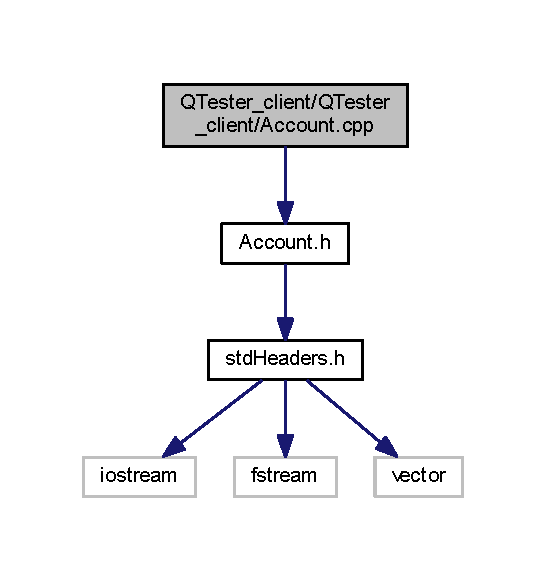
\includegraphics[width=262pt]{d5/df0/_account_8cpp__incl}
\end{center}
\end{figure}

\hypertarget{_account_8h}{}\section{Файл Q\+Tester\+\_\+client/\+Q\+Tester\+\_\+client/\+Account.h}
\label{_account_8h}\index{Q\+Tester\+\_\+client/\+Q\+Tester\+\_\+client/\+Account.\+h@{Q\+Tester\+\_\+client/\+Q\+Tester\+\_\+client/\+Account.\+h}}
{\ttfamily \#include \char`\"{}std\+Headers.\+h\char`\"{}}\\*
Граф включаемых заголовочных файлов для Account.\+h\+:\nopagebreak
\begin{figure}[H]
\begin{center}
\leavevmode
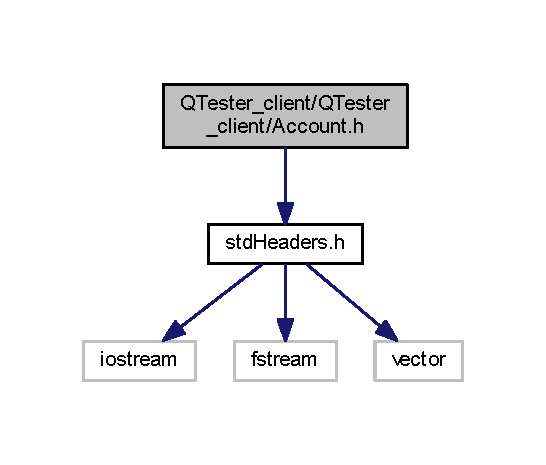
\includegraphics[width=262pt]{d6/d7d/_account_8h__incl}
\end{center}
\end{figure}
Граф файлов, в которые включается этот файл\+:\nopagebreak
\begin{figure}[H]
\begin{center}
\leavevmode
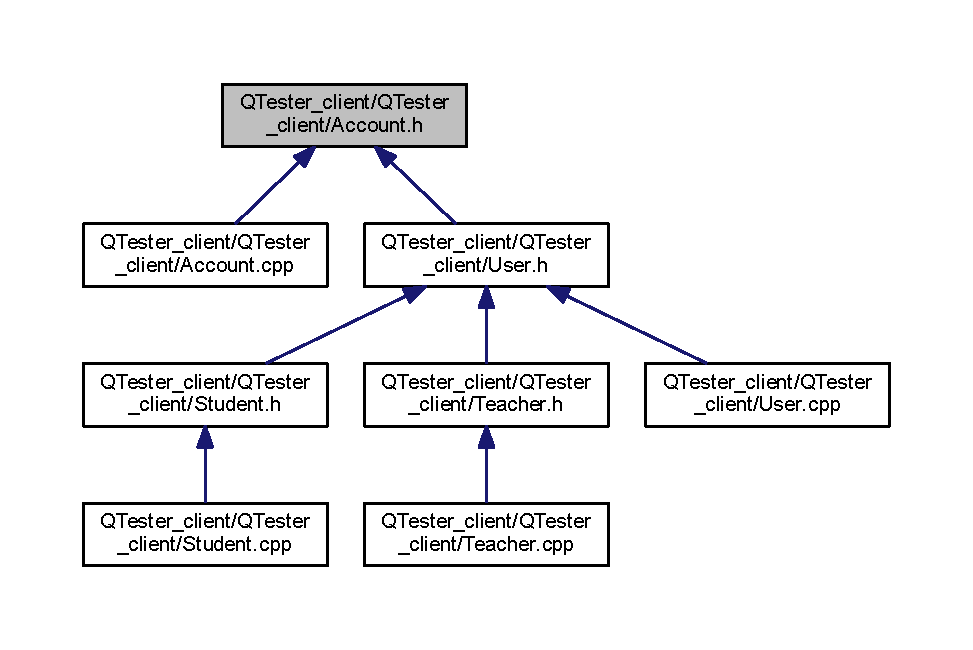
\includegraphics[width=350pt]{dc/d23/_account_8h__dep__incl}
\end{center}
\end{figure}
\subsection*{Классы}
\begin{DoxyCompactItemize}
\item 
class \hyperlink{class_account}{Account}
\end{DoxyCompactItemize}

\hypertarget{_administrator_8cpp}{}\section{Файл Q\+Tester\+\_\+client/\+Q\+Tester\+\_\+client/\+Administrator.cpp}
\label{_administrator_8cpp}\index{Q\+Tester\+\_\+client/\+Q\+Tester\+\_\+client/\+Administrator.\+cpp@{Q\+Tester\+\_\+client/\+Q\+Tester\+\_\+client/\+Administrator.\+cpp}}
{\ttfamily \#include \char`\"{}Administrator.\+h\char`\"{}}\\*
Граф включаемых заголовочных файлов для Administrator.\+cpp\+:\nopagebreak
\begin{figure}[H]
\begin{center}
\leavevmode
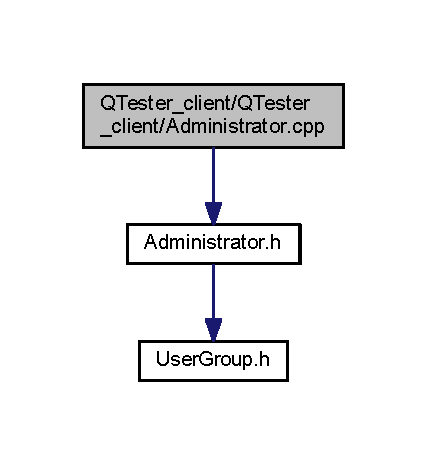
\includegraphics[width=205pt]{d6/d20/_administrator_8cpp__incl}
\end{center}
\end{figure}

\hypertarget{_administrator_8h}{}\section{Файл Q\+Tester\+\_\+client/\+Q\+Tester\+\_\+client/\+Administrator.h}
\label{_administrator_8h}\index{Q\+Tester\+\_\+client/\+Q\+Tester\+\_\+client/\+Administrator.\+h@{Q\+Tester\+\_\+client/\+Q\+Tester\+\_\+client/\+Administrator.\+h}}
{\ttfamily \#include \char`\"{}User\+Group.\+h\char`\"{}}\\*
Граф включаемых заголовочных файлов для Administrator.\+h\+:\nopagebreak
\begin{figure}[H]
\begin{center}
\leavevmode
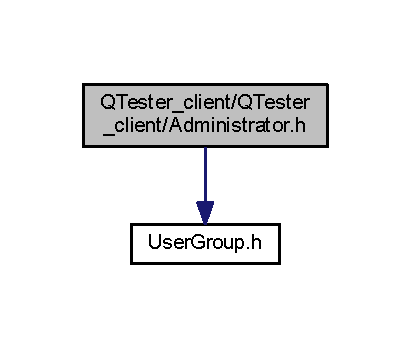
\includegraphics[width=197pt]{d7/d47/_administrator_8h__incl}
\end{center}
\end{figure}
Граф файлов, в которые включается этот файл\+:\nopagebreak
\begin{figure}[H]
\begin{center}
\leavevmode
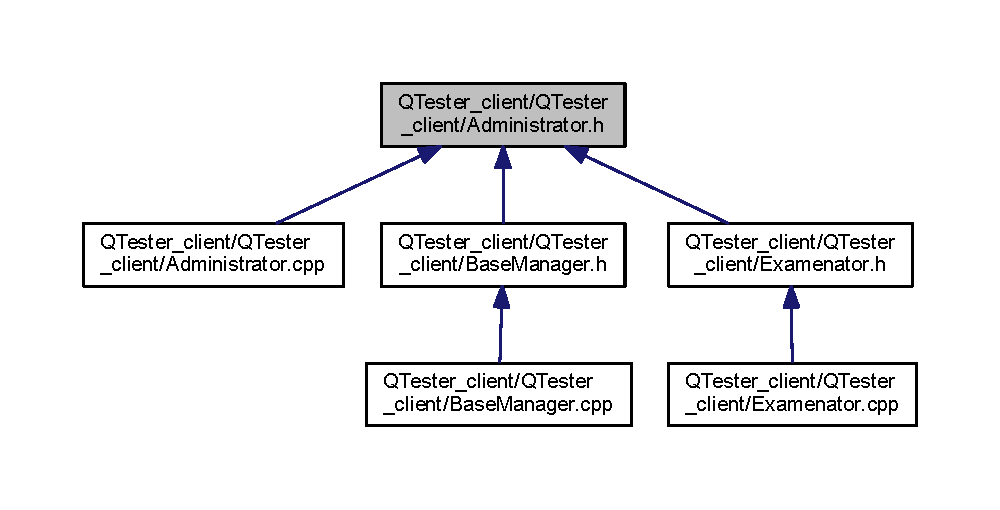
\includegraphics[width=350pt]{d7/db1/_administrator_8h__dep__incl}
\end{center}
\end{figure}
\subsection*{Классы}
\begin{DoxyCompactItemize}
\item 
class \hyperlink{class_administrator}{Administrator}
\end{DoxyCompactItemize}

\hypertarget{_base_manager_8cpp}{}\section{Файл Q\+Tester\+\_\+client/\+Q\+Tester\+\_\+client/\+Base\+Manager.cpp}
\label{_base_manager_8cpp}\index{Q\+Tester\+\_\+client/\+Q\+Tester\+\_\+client/\+Base\+Manager.\+cpp@{Q\+Tester\+\_\+client/\+Q\+Tester\+\_\+client/\+Base\+Manager.\+cpp}}
{\ttfamily \#include \char`\"{}Base\+Manager.\+h\char`\"{}}\\*
Граф включаемых заголовочных файлов для Base\+Manager.\+cpp\+:\nopagebreak
\begin{figure}[H]
\begin{center}
\leavevmode
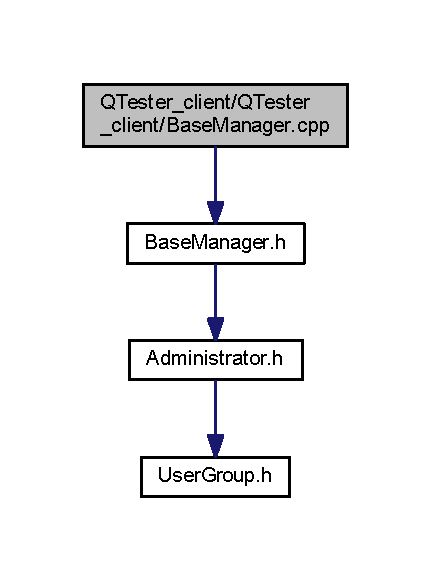
\includegraphics[width=207pt]{da/d40/_base_manager_8cpp__incl}
\end{center}
\end{figure}

\hypertarget{_base_manager_8h}{}\section{Файл Q\+Tester\+\_\+client/\+Q\+Tester\+\_\+client/\+Base\+Manager.h}
\label{_base_manager_8h}\index{Q\+Tester\+\_\+client/\+Q\+Tester\+\_\+client/\+Base\+Manager.\+h@{Q\+Tester\+\_\+client/\+Q\+Tester\+\_\+client/\+Base\+Manager.\+h}}
{\ttfamily \#include \char`\"{}Administrator.\+h\char`\"{}}\\*
Граф включаемых заголовочных файлов для Base\+Manager.\+h\+:\nopagebreak
\begin{figure}[H]
\begin{center}
\leavevmode
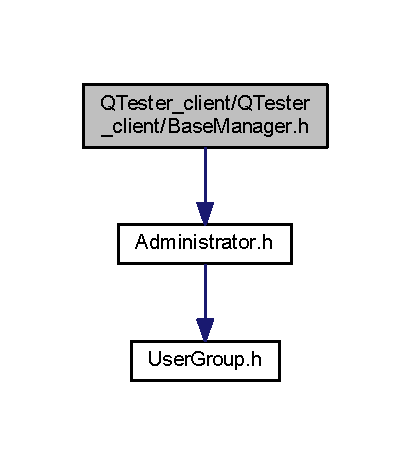
\includegraphics[width=197pt]{d5/de3/_base_manager_8h__incl}
\end{center}
\end{figure}
Граф файлов, в которые включается этот файл\+:\nopagebreak
\begin{figure}[H]
\begin{center}
\leavevmode
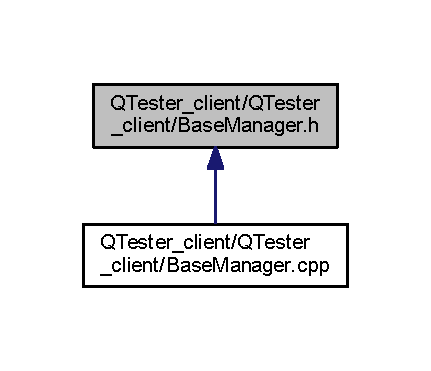
\includegraphics[width=207pt]{db/d4a/_base_manager_8h__dep__incl}
\end{center}
\end{figure}
\subsection*{Классы}
\begin{DoxyCompactItemize}
\item 
class \hyperlink{class_base_manager}{Base\+Manager}
\end{DoxyCompactItemize}

\hypertarget{_examenator_8cpp}{}\section{Файл Q\+Tester\+\_\+client/\+Q\+Tester\+\_\+client/\+Examenator.cpp}
\label{_examenator_8cpp}\index{Q\+Tester\+\_\+client/\+Q\+Tester\+\_\+client/\+Examenator.\+cpp@{Q\+Tester\+\_\+client/\+Q\+Tester\+\_\+client/\+Examenator.\+cpp}}
{\ttfamily \#include \char`\"{}Examenator.\+h\char`\"{}}\\*
Граф включаемых заголовочных файлов для Examenator.\+cpp\+:\nopagebreak
\begin{figure}[H]
\begin{center}
\leavevmode
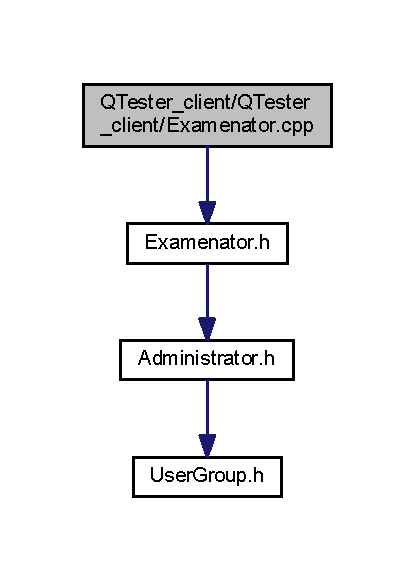
\includegraphics[width=199pt]{d8/df2/_examenator_8cpp__incl}
\end{center}
\end{figure}

\hypertarget{_examenator_8h}{}\section{Файл Q\+Tester\+\_\+client/\+Q\+Tester\+\_\+client/\+Examenator.h}
\label{_examenator_8h}\index{Q\+Tester\+\_\+client/\+Q\+Tester\+\_\+client/\+Examenator.\+h@{Q\+Tester\+\_\+client/\+Q\+Tester\+\_\+client/\+Examenator.\+h}}
{\ttfamily \#include \char`\"{}Administrator.\+h\char`\"{}}\\*
Граф включаемых заголовочных файлов для Examenator.\+h\+:\nopagebreak
\begin{figure}[H]
\begin{center}
\leavevmode
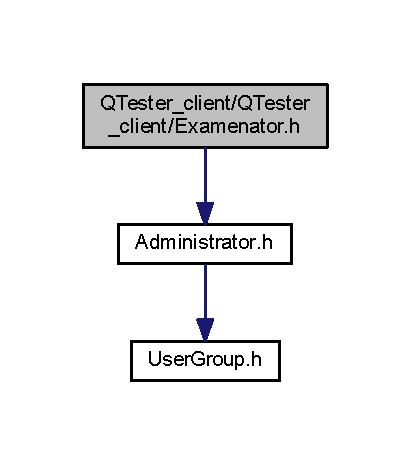
\includegraphics[width=197pt]{de/d86/_examenator_8h__incl}
\end{center}
\end{figure}
Граф файлов, в которые включается этот файл\+:\nopagebreak
\begin{figure}[H]
\begin{center}
\leavevmode
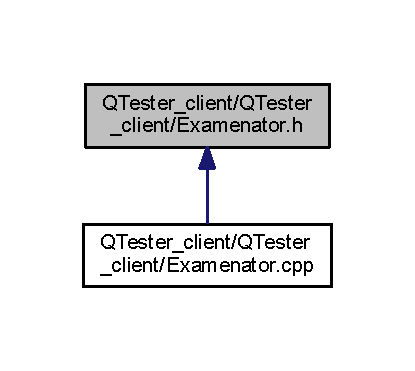
\includegraphics[width=199pt]{d2/db3/_examenator_8h__dep__incl}
\end{center}
\end{figure}
\subsection*{Классы}
\begin{DoxyCompactItemize}
\item 
class \hyperlink{class_examenator}{Examenator}
\end{DoxyCompactItemize}

\hypertarget{_examiner_8cpp}{}\section{Файл Q\+Tester\+\_\+client/\+Q\+Tester\+\_\+client/\+Examiner.cpp}
\label{_examiner_8cpp}\index{Q\+Tester\+\_\+client/\+Q\+Tester\+\_\+client/\+Examiner.\+cpp@{Q\+Tester\+\_\+client/\+Q\+Tester\+\_\+client/\+Examiner.\+cpp}}
{\ttfamily \#include \char`\"{}Examiner.\+h\char`\"{}}\\*
Граф включаемых заголовочных файлов для Examiner.\+cpp\+:\nopagebreak
\begin{figure}[H]
\begin{center}
\leavevmode
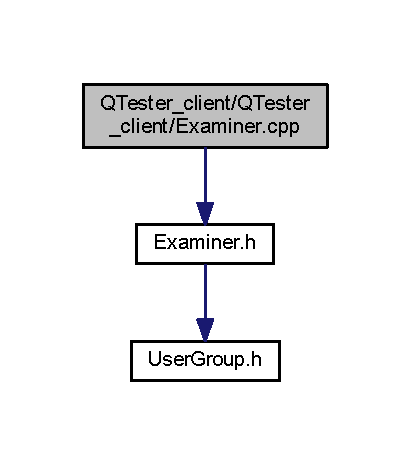
\includegraphics[width=197pt]{d2/d76/_examiner_8cpp__incl}
\end{center}
\end{figure}

\hypertarget{_examiner_8h}{}\section{Файл Q\+Tester\+\_\+client/\+Q\+Tester\+\_\+client/\+Examiner.h}
\label{_examiner_8h}\index{Q\+Tester\+\_\+client/\+Q\+Tester\+\_\+client/\+Examiner.\+h@{Q\+Tester\+\_\+client/\+Q\+Tester\+\_\+client/\+Examiner.\+h}}
{\ttfamily \#include \char`\"{}User\+Group.\+h\char`\"{}}\\*
Граф включаемых заголовочных файлов для Examiner.\+h\+:\nopagebreak
\begin{figure}[H]
\begin{center}
\leavevmode
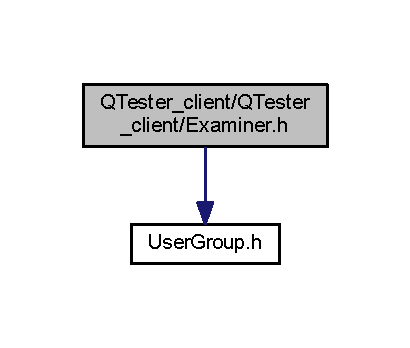
\includegraphics[width=197pt]{d6/de5/_examiner_8h__incl}
\end{center}
\end{figure}
Граф файлов, в которые включается этот файл\+:\nopagebreak
\begin{figure}[H]
\begin{center}
\leavevmode
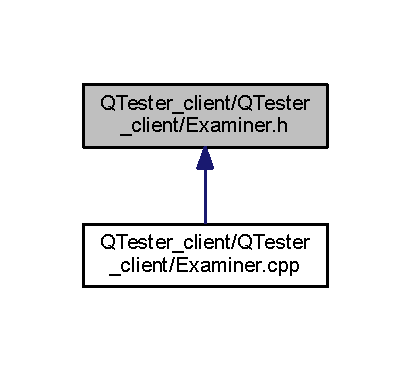
\includegraphics[width=197pt]{d9/d93/_examiner_8h__dep__incl}
\end{center}
\end{figure}
\subsection*{Классы}
\begin{DoxyCompactItemize}
\item 
class \hyperlink{class_examiner}{Examiner}
\end{DoxyCompactItemize}

\hypertarget{main_8cpp}{}\section{Файл Q\+Tester\+\_\+client/\+Q\+Tester\+\_\+client/main.cpp}
\label{main_8cpp}\index{Q\+Tester\+\_\+client/\+Q\+Tester\+\_\+client/main.\+cpp@{Q\+Tester\+\_\+client/\+Q\+Tester\+\_\+client/main.\+cpp}}
{\ttfamily \#include $<$Qt\+Core/\+Q\+Core\+Application$>$}\\*
Граф включаемых заголовочных файлов для main.\+cpp\+:\nopagebreak
\begin{figure}[H]
\begin{center}
\leavevmode
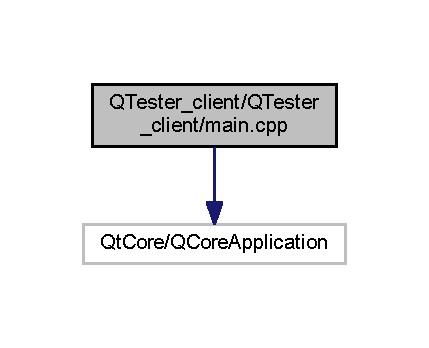
\includegraphics[width=206pt]{da/dce/main_8cpp__incl}
\end{center}
\end{figure}
\subsection*{Функции}
\begin{DoxyCompactItemize}
\item 
int \hyperlink{main_8cpp_a0ddf1224851353fc92bfbff6f499fa97}{main} (int argc, char $\ast$argv\mbox{[}$\,$\mbox{]})
\end{DoxyCompactItemize}


\subsection{Функции}
\hypertarget{main_8cpp_a0ddf1224851353fc92bfbff6f499fa97}{}\index{main.\+cpp@{main.\+cpp}!main@{main}}
\index{main@{main}!main.\+cpp@{main.\+cpp}}
\subsubsection[{main}]{\setlength{\rightskip}{0pt plus 5cm}int main (
\begin{DoxyParamCaption}
\item[{int}]{argc, }
\item[{char $\ast$}]{argv\mbox{[}$\,$\mbox{]}}
\end{DoxyParamCaption}
)}\label{main_8cpp_a0ddf1224851353fc92bfbff6f499fa97}


См. определение в файле main.\+cpp строка 4


\hypertarget{_s_q_lite_mgr_8cpp}{}\section{Файл Q\+Tester\+\_\+client/\+Q\+Tester\+\_\+client/\+S\+Q\+Lite\+Mgr.cpp}
\label{_s_q_lite_mgr_8cpp}\index{Q\+Tester\+\_\+client/\+Q\+Tester\+\_\+client/\+S\+Q\+Lite\+Mgr.\+cpp@{Q\+Tester\+\_\+client/\+Q\+Tester\+\_\+client/\+S\+Q\+Lite\+Mgr.\+cpp}}
{\ttfamily \#include \char`\"{}S\+Q\+Lite\+Mgr.\+h\char`\"{}}\\*
Граф включаемых заголовочных файлов для S\+Q\+Lite\+Mgr.\+cpp\+:\nopagebreak
\begin{figure}[H]
\begin{center}
\leavevmode
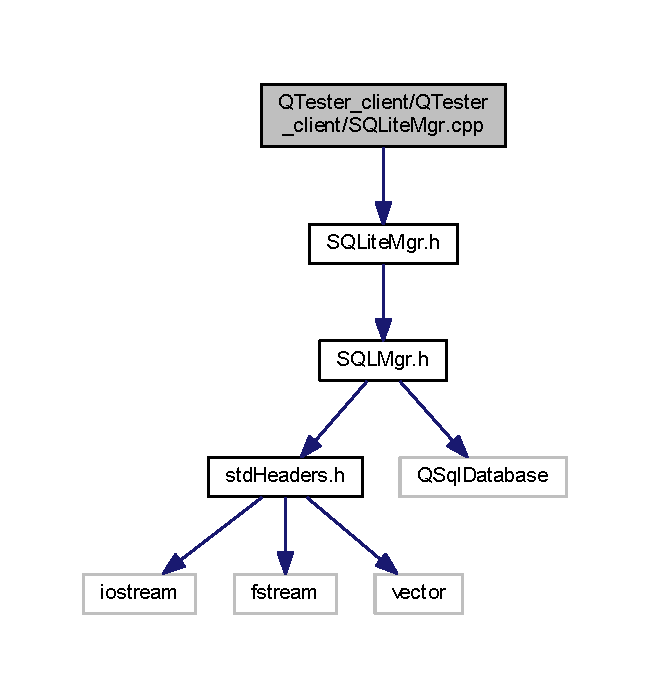
\includegraphics[width=312pt]{d1/d93/_s_q_lite_mgr_8cpp__incl}
\end{center}
\end{figure}

\hypertarget{_s_q_lite_mgr_8h}{}\section{Файл Q\+Tester\+\_\+client/\+Q\+Tester\+\_\+client/\+S\+Q\+Lite\+Mgr.h}
\label{_s_q_lite_mgr_8h}\index{Q\+Tester\+\_\+client/\+Q\+Tester\+\_\+client/\+S\+Q\+Lite\+Mgr.\+h@{Q\+Tester\+\_\+client/\+Q\+Tester\+\_\+client/\+S\+Q\+Lite\+Mgr.\+h}}
{\ttfamily \#include \char`\"{}S\+Q\+L\+Mgr.\+h\char`\"{}}\\*
Граф включаемых заголовочных файлов для S\+Q\+Lite\+Mgr.\+h\+:\nopagebreak
\begin{figure}[H]
\begin{center}
\leavevmode
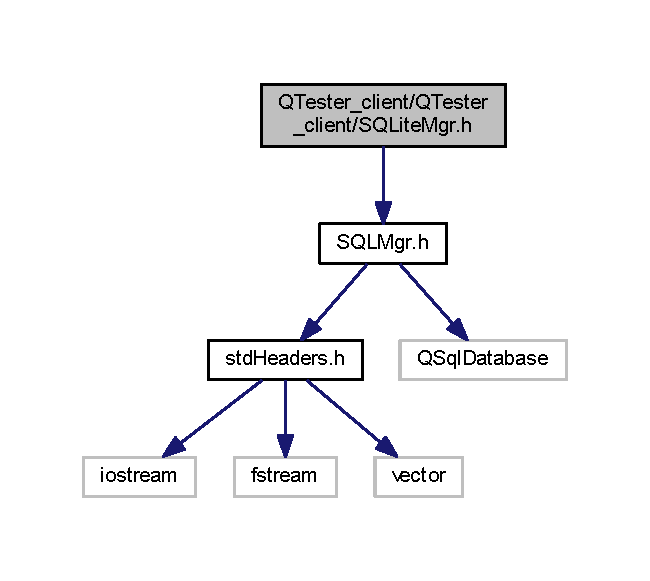
\includegraphics[width=312pt]{d1/dcf/_s_q_lite_mgr_8h__incl}
\end{center}
\end{figure}
Граф файлов, в которые включается этот файл\+:\nopagebreak
\begin{figure}[H]
\begin{center}
\leavevmode
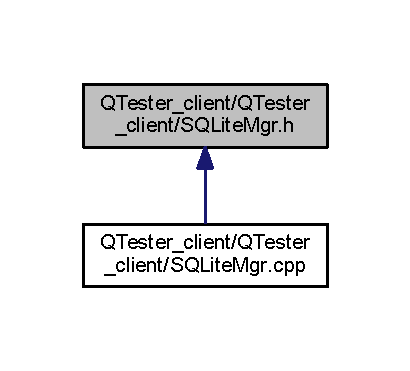
\includegraphics[width=197pt]{de/d16/_s_q_lite_mgr_8h__dep__incl}
\end{center}
\end{figure}
\subsection*{Классы}
\begin{DoxyCompactItemize}
\item 
class \hyperlink{class_s_q_lite_mgr}{S\+Q\+Lite\+Mgr}
\end{DoxyCompactItemize}

\hypertarget{_s_q_l_mgr_8cpp}{}\section{Файл Q\+Tester\+\_\+client/\+Q\+Tester\+\_\+client/\+S\+Q\+L\+Mgr.cpp}
\label{_s_q_l_mgr_8cpp}\index{Q\+Tester\+\_\+client/\+Q\+Tester\+\_\+client/\+S\+Q\+L\+Mgr.\+cpp@{Q\+Tester\+\_\+client/\+Q\+Tester\+\_\+client/\+S\+Q\+L\+Mgr.\+cpp}}
{\ttfamily \#include \char`\"{}S\+Q\+L\+Mgr.\+h\char`\"{}}\\*
Граф включаемых заголовочных файлов для S\+Q\+L\+Mgr.\+cpp\+:\nopagebreak
\begin{figure}[H]
\begin{center}
\leavevmode
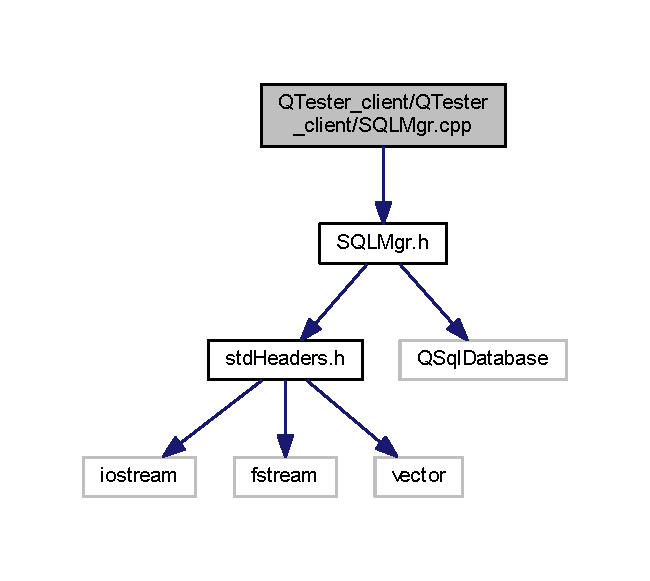
\includegraphics[width=312pt]{dd/dda/_s_q_l_mgr_8cpp__incl}
\end{center}
\end{figure}

\hypertarget{_s_q_l_mgr_8h}{}\section{Файл Q\+Tester\+\_\+client/\+Q\+Tester\+\_\+client/\+S\+Q\+L\+Mgr.h}
\label{_s_q_l_mgr_8h}\index{Q\+Tester\+\_\+client/\+Q\+Tester\+\_\+client/\+S\+Q\+L\+Mgr.\+h@{Q\+Tester\+\_\+client/\+Q\+Tester\+\_\+client/\+S\+Q\+L\+Mgr.\+h}}
{\ttfamily \#include \char`\"{}std\+Headers.\+h\char`\"{}}\\*
{\ttfamily \#include $<$Q\+Sql\+Database$>$}\\*
Граф включаемых заголовочных файлов для S\+Q\+L\+Mgr.\+h\+:\nopagebreak
\begin{figure}[H]
\begin{center}
\leavevmode
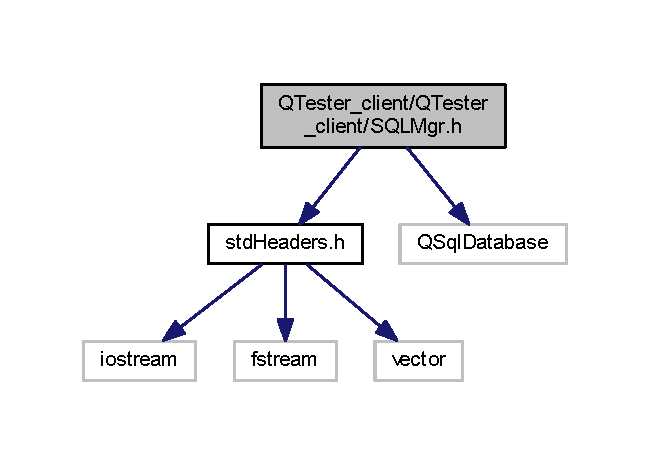
\includegraphics[width=312pt]{de/d88/_s_q_l_mgr_8h__incl}
\end{center}
\end{figure}
Граф файлов, в которые включается этот файл\+:\nopagebreak
\begin{figure}[H]
\begin{center}
\leavevmode
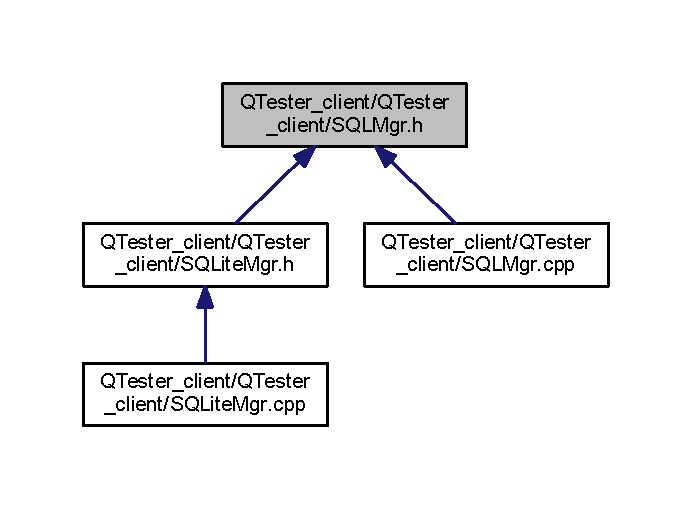
\includegraphics[width=332pt]{d9/d28/_s_q_l_mgr_8h__dep__incl}
\end{center}
\end{figure}
\subsection*{Классы}
\begin{DoxyCompactItemize}
\item 
class \hyperlink{class_s_q_l_mgr}{S\+Q\+L\+Mgr}
\end{DoxyCompactItemize}

\hypertarget{std_headers_8cpp}{}\section{Файл Q\+Tester\+\_\+client/\+Q\+Tester\+\_\+client/std\+Headers.cpp}
\label{std_headers_8cpp}\index{Q\+Tester\+\_\+client/\+Q\+Tester\+\_\+client/std\+Headers.\+cpp@{Q\+Tester\+\_\+client/\+Q\+Tester\+\_\+client/std\+Headers.\+cpp}}
{\ttfamily \#include \char`\"{}std\+Headers.\+h\char`\"{}}\\*
Граф включаемых заголовочных файлов для std\+Headers.\+cpp\+:\nopagebreak
\begin{figure}[H]
\begin{center}
\leavevmode
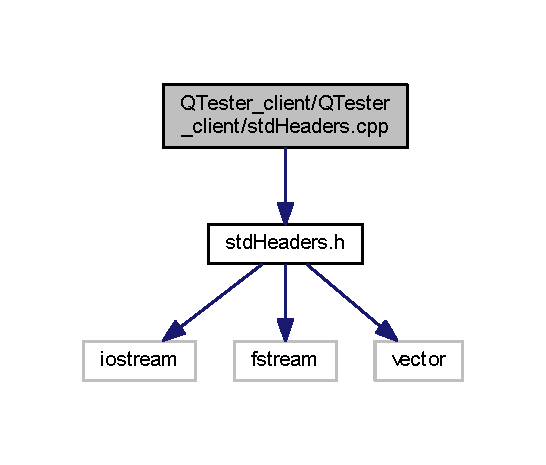
\includegraphics[width=262pt]{d7/d3a/std_headers_8cpp__incl}
\end{center}
\end{figure}

\hypertarget{std_headers_8h}{}\section{Файл Q\+Tester\+\_\+client/\+Q\+Tester\+\_\+client/std\+Headers.h}
\label{std_headers_8h}\index{Q\+Tester\+\_\+client/\+Q\+Tester\+\_\+client/std\+Headers.\+h@{Q\+Tester\+\_\+client/\+Q\+Tester\+\_\+client/std\+Headers.\+h}}
{\ttfamily \#include $<$iostream$>$}\\*
{\ttfamily \#include $<$fstream$>$}\\*
{\ttfamily \#include $<$vector$>$}\\*
Граф включаемых заголовочных файлов для std\+Headers.\+h\+:\nopagebreak
\begin{figure}[H]
\begin{center}
\leavevmode
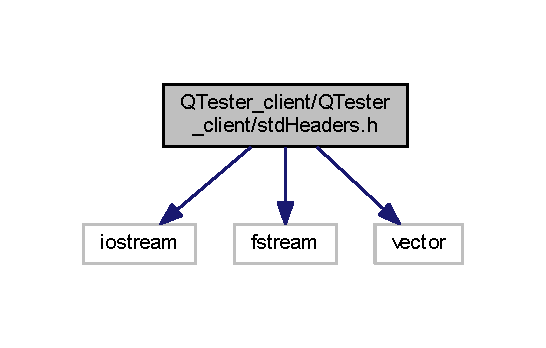
\includegraphics[width=262pt]{d0/d40/std_headers_8h__incl}
\end{center}
\end{figure}
Граф файлов, в которые включается этот файл\+:\nopagebreak
\begin{figure}[H]
\begin{center}
\leavevmode
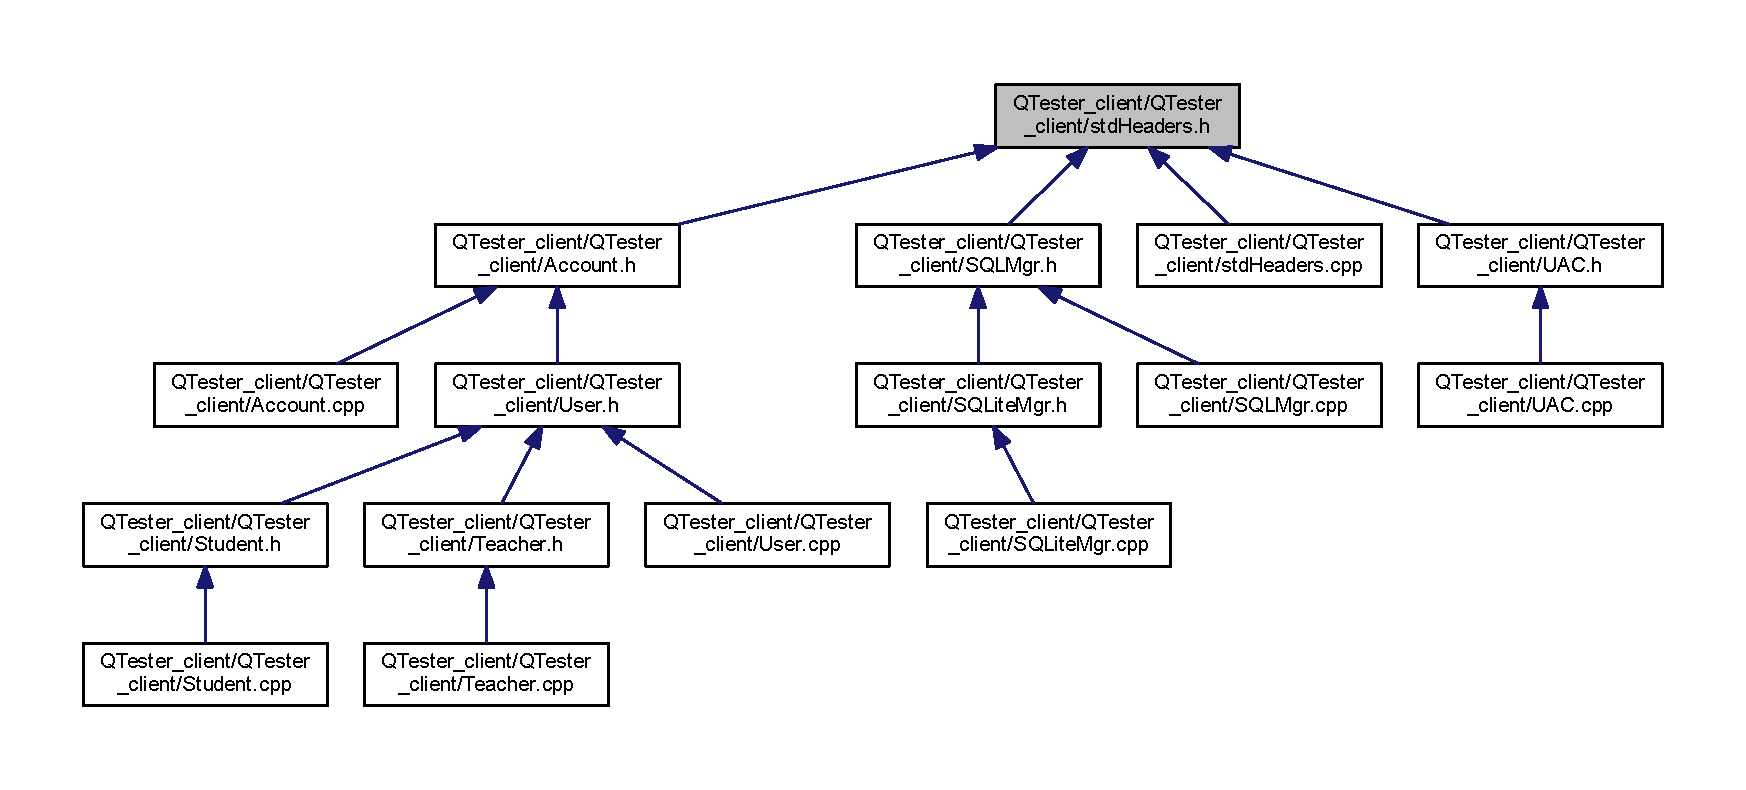
\includegraphics[width=350pt]{d5/d6e/std_headers_8h__dep__incl}
\end{center}
\end{figure}

\hypertarget{_student_8cpp}{}\section{Файл Q\+Tester\+\_\+client/\+Q\+Tester\+\_\+client/\+Student.cpp}
\label{_student_8cpp}\index{Q\+Tester\+\_\+client/\+Q\+Tester\+\_\+client/\+Student.\+cpp@{Q\+Tester\+\_\+client/\+Q\+Tester\+\_\+client/\+Student.\+cpp}}
{\ttfamily \#include \char`\"{}Student.\+h\char`\"{}}\\*
Граф включаемых заголовочных файлов для Student.\+cpp\+:\nopagebreak
\begin{figure}[H]
\begin{center}
\leavevmode
\includegraphics[width=262pt]{d3/d14/_student_8cpp__incl}
\end{center}
\end{figure}

\hypertarget{_student_8h}{}\section{Файл Q\+Tester\+\_\+client/\+Q\+Tester\+\_\+client/\+Student.h}
\label{_student_8h}\index{Q\+Tester\+\_\+client/\+Q\+Tester\+\_\+client/\+Student.\+h@{Q\+Tester\+\_\+client/\+Q\+Tester\+\_\+client/\+Student.\+h}}
{\ttfamily \#include \char`\"{}User.\+h\char`\"{}}\\*
Граф включаемых заголовочных файлов для Student.\+h\+:\nopagebreak
\begin{figure}[H]
\begin{center}
\leavevmode
\includegraphics[width=262pt]{dc/d98/_student_8h__incl}
\end{center}
\end{figure}
Граф файлов, в которые включается этот файл\+:\nopagebreak
\begin{figure}[H]
\begin{center}
\leavevmode
\includegraphics[width=197pt]{d6/de7/_student_8h__dep__incl}
\end{center}
\end{figure}
\subsection*{Классы}
\begin{DoxyCompactItemize}
\item 
class \hyperlink{class_student}{Student}
\end{DoxyCompactItemize}

\hypertarget{_teacher_8cpp}{}\section{Файл Q\+Tester\+\_\+client/\+Q\+Tester\+\_\+client/\+Teacher.cpp}
\label{_teacher_8cpp}\index{Q\+Tester\+\_\+client/\+Q\+Tester\+\_\+client/\+Teacher.\+cpp@{Q\+Tester\+\_\+client/\+Q\+Tester\+\_\+client/\+Teacher.\+cpp}}
{\ttfamily \#include \char`\"{}Teacher.\+h\char`\"{}}\\*
Граф включаемых заголовочных файлов для Teacher.\+cpp\+:\nopagebreak
\begin{figure}[H]
\begin{center}
\leavevmode
\includegraphics[width=262pt]{d1/dc2/_teacher_8cpp__incl}
\end{center}
\end{figure}

\hypertarget{_teacher_8h}{}\section{Файл Q\+Tester\+\_\+client/\+Q\+Tester\+\_\+client/\+Teacher.h}
\label{_teacher_8h}\index{Q\+Tester\+\_\+client/\+Q\+Tester\+\_\+client/\+Teacher.\+h@{Q\+Tester\+\_\+client/\+Q\+Tester\+\_\+client/\+Teacher.\+h}}
{\ttfamily \#include \char`\"{}User.\+h\char`\"{}}\\*
Граф включаемых заголовочных файлов для Teacher.\+h\+:\nopagebreak
\begin{figure}[H]
\begin{center}
\leavevmode
\includegraphics[width=262pt]{d5/d51/_teacher_8h__incl}
\end{center}
\end{figure}
Граф файлов, в которые включается этот файл\+:\nopagebreak
\begin{figure}[H]
\begin{center}
\leavevmode
\includegraphics[width=197pt]{d7/d10/_teacher_8h__dep__incl}
\end{center}
\end{figure}
\subsection*{Классы}
\begin{DoxyCompactItemize}
\item 
class \hyperlink{class_teacher}{Teacher}
\end{DoxyCompactItemize}

\hypertarget{_tester_8cpp}{}\section{Файл Q\+Tester\+\_\+client/\+Q\+Tester\+\_\+client/\+Tester.cpp}
\label{_tester_8cpp}\index{Q\+Tester\+\_\+client/\+Q\+Tester\+\_\+client/\+Tester.\+cpp@{Q\+Tester\+\_\+client/\+Q\+Tester\+\_\+client/\+Tester.\+cpp}}
{\ttfamily \#include \char`\"{}Tester.\+h\char`\"{}}\\*
Граф включаемых заголовочных файлов для Tester.\+cpp\+:\nopagebreak
\begin{figure}[H]
\begin{center}
\leavevmode
\includegraphics[width=197pt]{d4/d66/_tester_8cpp__incl}
\end{center}
\end{figure}

\hypertarget{_tester_8h}{}\section{Файл Q\+Tester\+\_\+client/\+Q\+Tester\+\_\+client/\+Tester.h}
\label{_tester_8h}\index{Q\+Tester\+\_\+client/\+Q\+Tester\+\_\+client/\+Tester.\+h@{Q\+Tester\+\_\+client/\+Q\+Tester\+\_\+client/\+Tester.\+h}}
Граф файлов, в которые включается этот файл\+:\nopagebreak
\begin{figure}[H]
\begin{center}
\leavevmode
\includegraphics[width=197pt]{da/dee/_tester_8h__dep__incl}
\end{center}
\end{figure}
\subsection*{Классы}
\begin{DoxyCompactItemize}
\item 
class \hyperlink{class_tester}{Tester}
\end{DoxyCompactItemize}

\hypertarget{_test_generator_8cpp}{}\section{Файл Q\+Tester\+\_\+client/\+Q\+Tester\+\_\+client/\+Test\+Generator.cpp}
\label{_test_generator_8cpp}\index{Q\+Tester\+\_\+client/\+Q\+Tester\+\_\+client/\+Test\+Generator.\+cpp@{Q\+Tester\+\_\+client/\+Q\+Tester\+\_\+client/\+Test\+Generator.\+cpp}}
{\ttfamily \#include \char`\"{}Test\+Generator.\+h\char`\"{}}\\*
Граф включаемых заголовочных файлов для Test\+Generator.\+cpp\+:\nopagebreak
\begin{figure}[H]
\begin{center}
\leavevmode
\includegraphics[width=208pt]{d6/d81/_test_generator_8cpp__incl}
\end{center}
\end{figure}

\hypertarget{_test_generator_8h}{}\section{Файл Q\+Tester\+\_\+client/\+Q\+Tester\+\_\+client/\+Test\+Generator.h}
\label{_test_generator_8h}\index{Q\+Tester\+\_\+client/\+Q\+Tester\+\_\+client/\+Test\+Generator.\+h@{Q\+Tester\+\_\+client/\+Q\+Tester\+\_\+client/\+Test\+Generator.\+h}}
Граф файлов, в которые включается этот файл\+:\nopagebreak
\begin{figure}[H]
\begin{center}
\leavevmode
\includegraphics[width=208pt]{d1/d09/_test_generator_8h__dep__incl}
\end{center}
\end{figure}
\subsection*{Классы}
\begin{DoxyCompactItemize}
\item 
class \hyperlink{class_test_generator}{Test\+Generator}
\end{DoxyCompactItemize}

\hypertarget{_u_a_c_8cpp}{}\section{Файл Q\+Tester\+\_\+client/\+Q\+Tester\+\_\+client/\+U\+A\+C.cpp}
\label{_u_a_c_8cpp}\index{Q\+Tester\+\_\+client/\+Q\+Tester\+\_\+client/\+U\+A\+C.\+cpp@{Q\+Tester\+\_\+client/\+Q\+Tester\+\_\+client/\+U\+A\+C.\+cpp}}
{\ttfamily \#include \char`\"{}U\+A\+C.\+h\char`\"{}}\\*
Граф включаемых заголовочных файлов для U\+A\+C.\+cpp\+:\nopagebreak
\begin{figure}[H]
\begin{center}
\leavevmode
\includegraphics[width=262pt]{d8/de5/_u_a_c_8cpp__incl}
\end{center}
\end{figure}

\hypertarget{_u_a_c_8h}{}\section{Файл Q\+Tester\+\_\+client/\+Q\+Tester\+\_\+client/\+U\+A\+C.h}
\label{_u_a_c_8h}\index{Q\+Tester\+\_\+client/\+Q\+Tester\+\_\+client/\+U\+A\+C.\+h@{Q\+Tester\+\_\+client/\+Q\+Tester\+\_\+client/\+U\+A\+C.\+h}}
{\ttfamily \#include $<$std\+Headers.\+h$>$}\\*
Граф включаемых заголовочных файлов для U\+A\+C.\+h\+:\nopagebreak
\begin{figure}[H]
\begin{center}
\leavevmode
\includegraphics[width=262pt]{dd/df2/_u_a_c_8h__incl}
\end{center}
\end{figure}
Граф файлов, в которые включается этот файл\+:\nopagebreak
\begin{figure}[H]
\begin{center}
\leavevmode
\includegraphics[width=197pt]{d1/d20/_u_a_c_8h__dep__incl}
\end{center}
\end{figure}
\subsection*{Классы}
\begin{DoxyCompactItemize}
\item 
class \hyperlink{class_u_a_c}{U\+A\+C}
\end{DoxyCompactItemize}

\hypertarget{_user_8cpp}{}\section{Файл Q\+Tester\+\_\+client/\+Q\+Tester\+\_\+client/\+User.cpp}
\label{_user_8cpp}\index{Q\+Tester\+\_\+client/\+Q\+Tester\+\_\+client/\+User.\+cpp@{Q\+Tester\+\_\+client/\+Q\+Tester\+\_\+client/\+User.\+cpp}}
{\ttfamily \#include \char`\"{}User.\+h\char`\"{}}\\*
Граф включаемых заголовочных файлов для User.\+cpp\+:\nopagebreak
\begin{figure}[H]
\begin{center}
\leavevmode
\includegraphics[width=262pt]{d5/de6/_user_8cpp__incl}
\end{center}
\end{figure}

\hypertarget{_user_8h}{}\section{Файл Q\+Tester\+\_\+client/\+Q\+Tester\+\_\+client/\+User.h}
\label{_user_8h}\index{Q\+Tester\+\_\+client/\+Q\+Tester\+\_\+client/\+User.\+h@{Q\+Tester\+\_\+client/\+Q\+Tester\+\_\+client/\+User.\+h}}
{\ttfamily \#include \char`\"{}Account.\+h\char`\"{}}\\*
Граф включаемых заголовочных файлов для User.\+h\+:\nopagebreak
\begin{figure}[H]
\begin{center}
\leavevmode
\includegraphics[width=262pt]{d5/de1/_user_8h__incl}
\end{center}
\end{figure}
Граф файлов, в которые включается этот файл\+:\nopagebreak
\begin{figure}[H]
\begin{center}
\leavevmode
\includegraphics[width=350pt]{d6/db5/_user_8h__dep__incl}
\end{center}
\end{figure}
\subsection*{Классы}
\begin{DoxyCompactItemize}
\item 
class \hyperlink{class_user}{User}
\end{DoxyCompactItemize}

\hypertarget{_user_group_8cpp}{}\section{Файл Q\+Tester\+\_\+client/\+Q\+Tester\+\_\+client/\+User\+Group.cpp}
\label{_user_group_8cpp}\index{Q\+Tester\+\_\+client/\+Q\+Tester\+\_\+client/\+User\+Group.\+cpp@{Q\+Tester\+\_\+client/\+Q\+Tester\+\_\+client/\+User\+Group.\+cpp}}
{\ttfamily \#include \char`\"{}User\+Group.\+h\char`\"{}}\\*
Граф включаемых заголовочных файлов для User\+Group.\+cpp\+:\nopagebreak
\begin{figure}[H]
\begin{center}
\leavevmode
\includegraphics[width=197pt]{d0/d12/_user_group_8cpp__incl}
\end{center}
\end{figure}

\hypertarget{_user_group_8h}{}\section{Файл Q\+Tester\+\_\+client/\+Q\+Tester\+\_\+client/\+User\+Group.h}
\label{_user_group_8h}\index{Q\+Tester\+\_\+client/\+Q\+Tester\+\_\+client/\+User\+Group.\+h@{Q\+Tester\+\_\+client/\+Q\+Tester\+\_\+client/\+User\+Group.\+h}}
Граф файлов, в которые включается этот файл\+:\nopagebreak
\begin{figure}[H]
\begin{center}
\leavevmode
\includegraphics[width=350pt]{d4/dc1/_user_group_8h__dep__incl}
\end{center}
\end{figure}
\subsection*{Классы}
\begin{DoxyCompactItemize}
\item 
class \hyperlink{class_user_group}{User\+Group}
\end{DoxyCompactItemize}

%--- End generated contents ---

% Index
\backmatter
\newpage
\phantomsection
\clearemptydoublepage
\addcontentsline{toc}{chapter}{Алфавитный указатель}
\printindex

\end{document}
